\documentclass[a4paper, titlepage]{article}

\usepackage[utf8]{inputenc}
\usepackage[T1]{fontenc}
\usepackage[margin=2.54cm]{geometry}
\usepackage[spanish, es-nodecimaldot]{babel}
\usepackage{hyperref}
\usepackage{url}
\usepackage{amsmath, amsthm, amssymb}
\usepackage{siunitx}
\usepackage[backend=biber, natbib=true, style=apa]{biblatex}
\usepackage[inline]{enumitem}
\usepackage{graphicx}
\usepackage{svg}
\usepackage{float}
\usepackage{minted}
\usepackage{xcolor}
\usepackage{csquotes}
\usepackage{mathtools}
\usepackage[title]{appendix}

\mathtoolsset{showonlyrefs}

\definecolor{codebg}{rgb}{0.95,0.95,0.95}
\setminted[python]{
    baselinestretch=1,
    fontsize=\footnotesize,
    linenos=true,
    bgcolor=codebg
}

\addbibresource{./main.bib}
\DeclareLanguageMapping{spanish}{spanish-apa}

\graphicspath{{./figures/}}

% Interlineado de 1.5
\renewcommand{\baselinestretch}{1.25}

\newtheorem{definition}{Definición}
\newtheorem{theorem}{Teorema}

\title{
    \centering
    
\includegraphics[width=0.2\textwidth]{utec} \\
    \vspace{24pt}
    Vibraciones mecánicas en estructuras de múltiples grados de libertad
}
\author{
    José Daniel Grayson Tejada \\
    \texttt{202410372} \and
    Diego Alonso Figueroa Winkelried \\
    \texttt{202410533} \and
    Joaquín Adrian Lopez Del Carpio \\
    \texttt{202410220} \and
    Gonzalo Andrés Valladolid Jimenes \\
    \texttt{202410186}
}

\begin{document}

\begin{titlepage}
\maketitle
\end{titlepage}

\addtocounter{page}{1}

\section{Introducción}

Las vibraciones mecánicas en edificios y otras estructuras constituyen una parte fundamental del área de estudio de la ingeniería civil. En particular, un caso de estudio frecuente en este campo es el análisis de las vibraciones en puentes. Es necesario realizar mediciones y estudios pertinentes de tanto dichas estructuras como los entornos sobre los que se encuentran con el fin de prevenir eventos catastróficos. El análisis de fenómenos tales como la resonancia son esenciales debido a sus implicaciones sobre la estabilidad de una estructura.

Un caso de accidente particularmente conocido es el del puente Yanango en Junín, ocurrido en noviembre de 2005. Accidentes de esta naturaleza demuestran la importancia de analizar las circunstancias a la que dichas estructuras se encuentran sometidas, ya sean propiamente estructurales o externas, como podrían ser las condiciones topográficas e hidrológicas \citep{mayhua}.

Para construir modelos físicos, tales como las vibraciones en puentes y estructuras afines, las ecuaciones diferenciales surgen como una herramienta fundamental. Nuestro principal objetivo será describir las vibraciones en puentes mediante la construcción de modelos físicos y matemáticos de ecuaciones diferenciales. Si bien varios de los aspectos a tratar ya han sido estudiados previamente por otros autores, la viabilidad de la propuesta se basa en tanto la generalización de algunos de estos conceptos como el planteamiento y estudio de un caso particular del cual se hará desarrollo posteriormente.
\section{Objetivos}

Este informe propone los siguientes objetivos para dirigir el desarrollo del presente trabajo:
p
\begin{enumerate}
    \item Modelar las vibraciones mecánicas de una estructura física de 3 grados de libertad mediante ecuaciones diferenciales.
    \item Generalizar el modelo matemático presentado a sistemas de múltiples grados de libertad (e.g. un edificio de \(n\) pisos).
    \item De ser posible, aplicar métodos de resolución de ecuaciones diferenciales para resolver explícitamente el modelo para estructuras de 2 pisos.
    \item Aplicar métodos numéricos para aproximar soluciones de la generalización del modelo para estructuras de \(n\) pisos.
    \item Emplear los resultados matemáticos obtenidos en el diseño de puentes y análisis estructural.
\end{enumerate}

\section{Marco teórico}

En esta sección, presentamos algunos términos, conceptos y teoremas que utilizaremos para construir el modelo matemático.

\subsection{Conceptos básicos}

La interacción de un objeto con las fuerzas que se ejercen sobre él se suele diagramar mediante un \textbf{diagrama de cuerpo libre} (DCL): ``un diagrama que muestra el cuerpo elegido solo, ``libre'' de su entorno, con vectores que muestren las magnitudes y direcciones de todas las fuerzas aplicadas sobre el cuerpo por todos los cuerpos que interactúan en él'' \citep{young}.

Por ejemplo, consideremos un objeto siendo arrastrado por el piso mediante una cuerda atada a un carro en movimiento. La figura \ref{fig:dcl-ejemplo} muestra esta situación y el DCL para este objeto siendo arrastrado.

\begin{figure}[h]
    \centering
    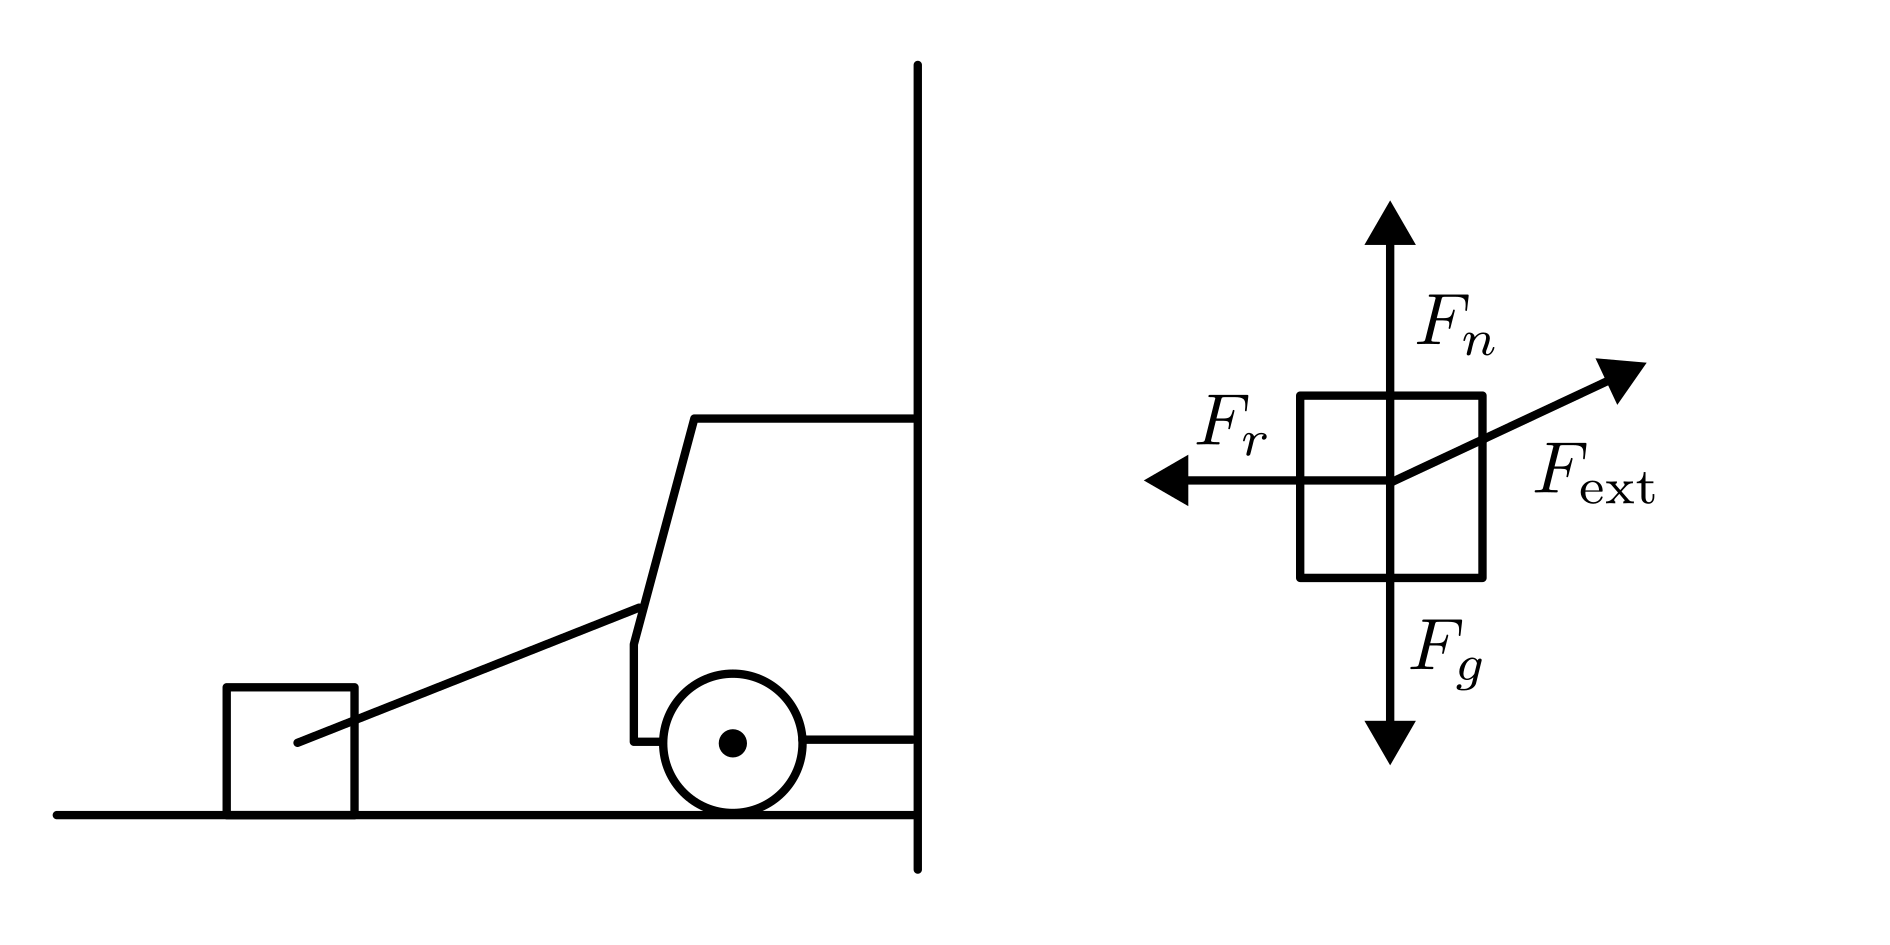
\includegraphics[width=0.6\textwidth]{dcl_ejemplo}
    \caption{Un ejemplo de sistema físico y el DCL de uno de sus elementos}
    \label{fig:dcl-ejemplo}
\end{figure}

\begin{definition}[amortiguamiento]
    En un sistema físico, el \textbf{amortiguamiento} (o amortiguación) es el fenómeno que ocurre en los objetos en movimiento, el cual \textit{disipa} la energía cinética.
\end{definition}

En sistemas físicos con velocidades relativamente bajas, se considera al amortiguamiento ejercido sobre un objeto como una fuerza proporcional y opuesta a su velocidad. \citet{rak} la definen mediante la relación
\[
    F_{a} = -cv
,\]
donde \(v\) es la velocidad del objeto (en \si{m/s}) y \(c\) es la \textbf{constante de amortiguamiento} (en \si{kg/s} y no negativa). Este tipo de amortiguamiento se denomina \textbf{amortiguamiento viscoso} \citep{rak}.

En la práctica, el amortiguamiento se suele definir mediante una \textbf{razón de amortiguamiento} (un coeficiente sin unidades), denotada por \(\zeta\). La constante de amortiguamiento \(c\) se puede calcular a partir la razón \(\zeta\) mediante
\[
    c = \zeta \left( 2\sqrt{mk} \right)
,\]
donde \(m\) es la masa del objeto y \(k\) su constante de elasticidad (concepto que será detallado más adelante en el marco teórico).

\subsection{Resultados y teoremas}

En primer lugar, es esencial para este trabajo enunciar la segunda ley de Newton, la cual parafraseamos del trabajo de \citet{young}.

\begin{theorem}[segunda ley de Newton]
    Sea \(m\) la masa (en \si{kg}) de un objeto, sea \(a\) su aceleración (en \si{m/s^2}) y sea \(\sum F_i\) (también llamada ``fuerza neta'') la suma de todas las fuerzas siendo aplicadas en dicho objeto en un instante particular.
    
        Entonces, en ese instante particular se cumple la ecuación
        \[
            \sum F_i = ma
        .\]
\end{theorem}

Esta ecuación será la base del modelo matemático que derivaremos.

La siguiente ley, también ampliamente conocida, nos permite caracterizar una de las fuerzas elásticas que actúan sobre las estructura que analizaremos más adelante. Parafraseando el trabajo de \citet{giuli}, enuncia lo siguiente:

\begin{theorem}[ley de Hooke]
    Sea \(x\) la posición (en metros) de un objeto con respecto a su punto de equilibrio, y sea \(F_e\) la \textbf{fuerza restauradora} ejercida sobre el objeto debido a su elasticidad.
    
        Entonces, se cumple que dicha fuerza restauradora es igual a
        \begin{equation}\label{eqn:hooke}
            F_{s} = -kx
        ,\end{equation}
        donde \(k\) (en \si{N/m}) es una constante no negativa llamada la \textbf{constante de elasticidad}.
\end{theorem}

En otras palabras, la fuerza restauradora ejercida sobre un objeto por elasticidad es proporcional a su posición con respecto a su punto de equilibrio.

En particular, \eqref{eqn:hooke} se puede aplicar al modelar la fuerza de restauración ejercida sobre una estructura que vibra horizontalmente, ya que se puede considerar que ``presenta un comportamiento elástico'' \citep{tarque}. En esta situación, se le llama a \(k\) la \textbf{rigidez} de la estructura.


\subsection{Métodos numéricos y Runge-Kutta}

Mientras que el modelado de fenómenos físicos por medio de ecuaciones diferenciales no es un proceso necesariamente complicado, su resolución a través de métodos analíticos exactos resulta, en muchos casos, una tarea muy difícil (o imposible). En este tipo de situaciones, los métodos numéricos son de gran utilidad para obtener soluciones aproximadas en lugar de analíticas \citep{reddy}.

Una familia de métodos numéricos que destacan por su simplicidad y efectividad son los métodos Runge-Kutta. Dentro de ellos, uno de los más frecuentemente usados es el método de \textbf{Runge-Kutta de orden 4} (RK4), el cual, parafraseando a \citet{suli}, consiste en aproximar iterativamente una EDO de la forma
\[
    y'(x) = f(x, y)
\]
a partir de un punto inicial \(y(t_0) = y_0\) mediante la fórmula
\[
    y_{n+1} = y_n + \frac{1}{6}h(k_1 + 2k_2 + 2k_3 + k_4)
,\]
donde los coeficientes \(k_1, k_2, k_3, k_4\) se calculan mediante
\begin{align*}
    k_1 &= f(x_n, y_n) \\
    k_2 &= f(x_n + \frac{1}{2}h, y_n + \frac{1}{2}hk_1) \\
    k_3 &= f(x_n + \frac{1}{2}h, y_n + \frac{1}{2}hk_2) \\
    k_4 &= f(x_n + h, y_n + hk_3) \\
.\end{align*}

Aunque esta formulación asume una sola EDO, el método de RK4 se puede extender para ser aplicado a sistemas de EDOs, lo cual será particularmente útil para este trabajo. Se incluye más información en el apéndice~\ref{appendix:rk4-systems}.
\section{Modelo matemático}

Previo a realizar el modelo para una cantidad arbitraria de pisos, modelaremos las ecuaciones diferenciales para estructuras de uno y tres pisos, de forma que los conceptos que usaremos serán introducidos de forma natural y progresiva.

Cabe resaltar que, como convención general, tomaremos al eje positivo de las posiciones \(u\) como la derecha.

\subsection{Para una estructura de un único grado de libertad}

Consideremos una estructura de un piso, como muestra la figura~\ref{fig:1-floor-diagram}, con masa \(m\) (en \si{kg}), rigidez lateral \(k\) (en \si{m/s^2}) y constante de amortiguamiento \(c\) (en \si{m/s}). Además, sea \(u\) la posición horizontal (en \si{m}) de la estructura con respecto a su estado de reposo, y consideremos que la estructura está siendo sometida a una fuerza de excitación externa \(P(t)\) (en \si{N}).

\begin{figure}[ht!]
    \centering
    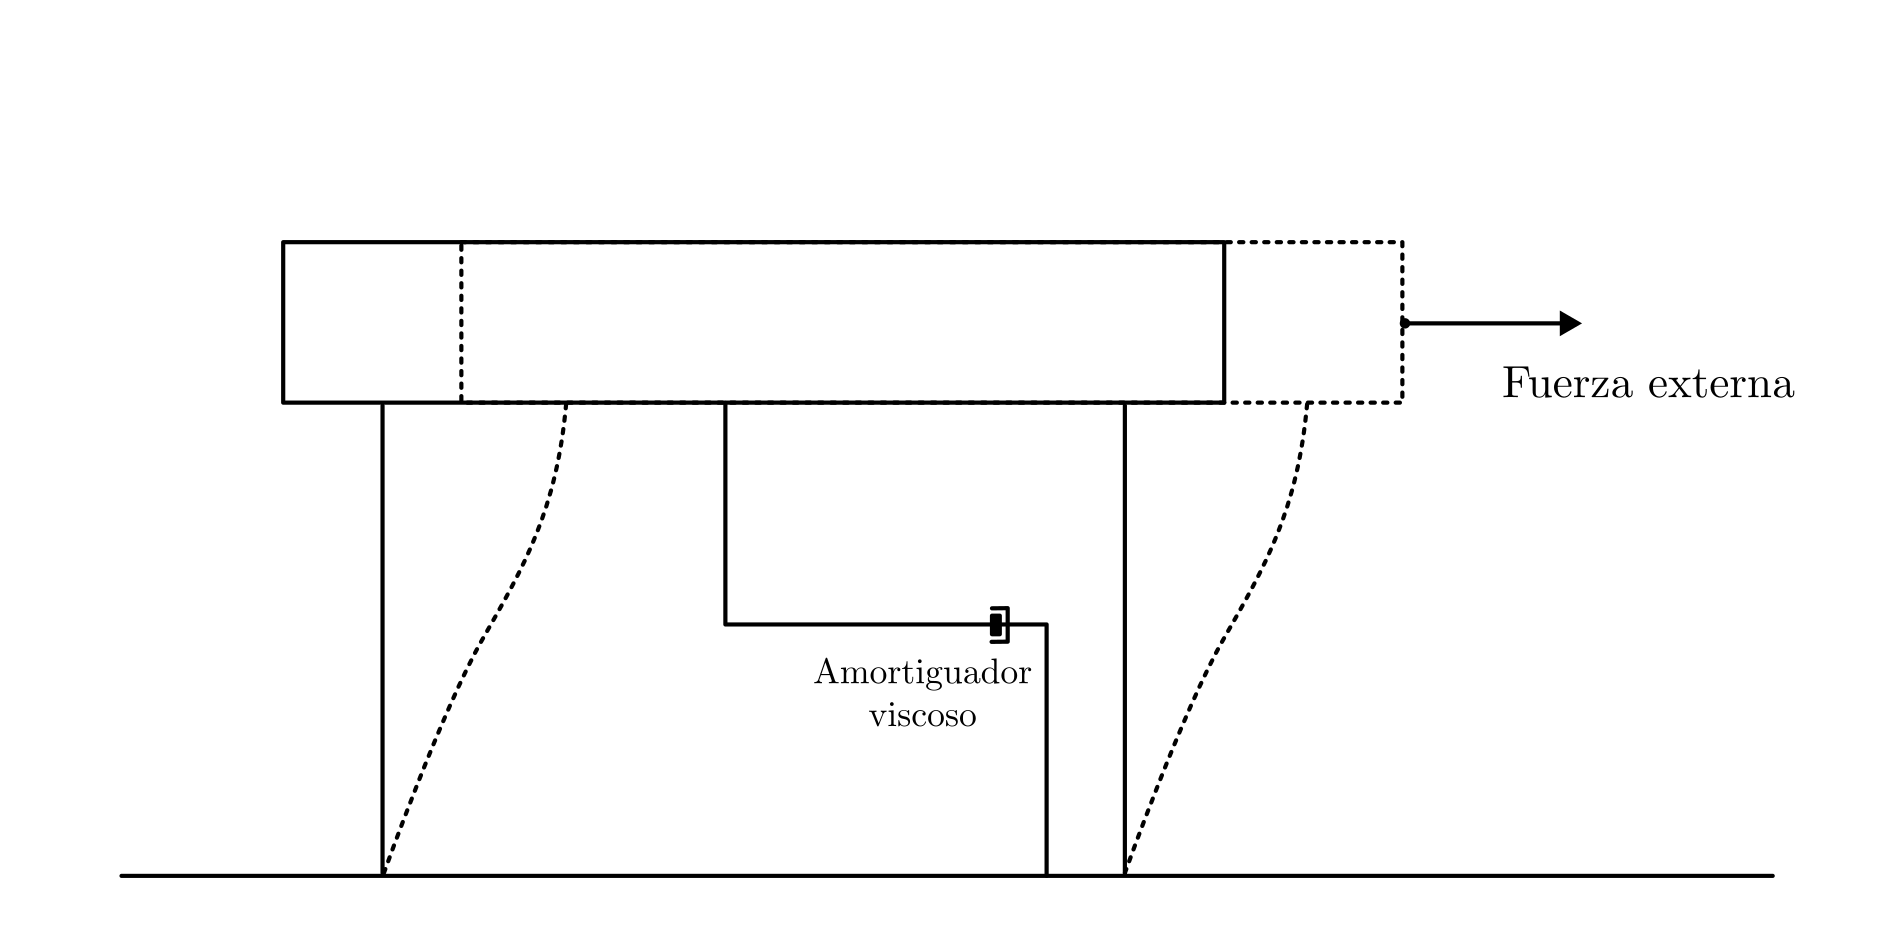
\includegraphics[width=0.8\textwidth]{diagrama_1_piso}
    \caption{Una estructura de un piso con amortiguamiento viscoso y una fuerza de excitación externa.}
    \label{fig:1-floor-diagram}
\end{figure}

Como solo tiene un piso, podemos considerar un único grado de libertad. El diagrama de cuerpo libre de la estructura se muestra en la figura~\ref{fig:1-floor-dcl}.

\begin{figure}[ht!]
    \centering
    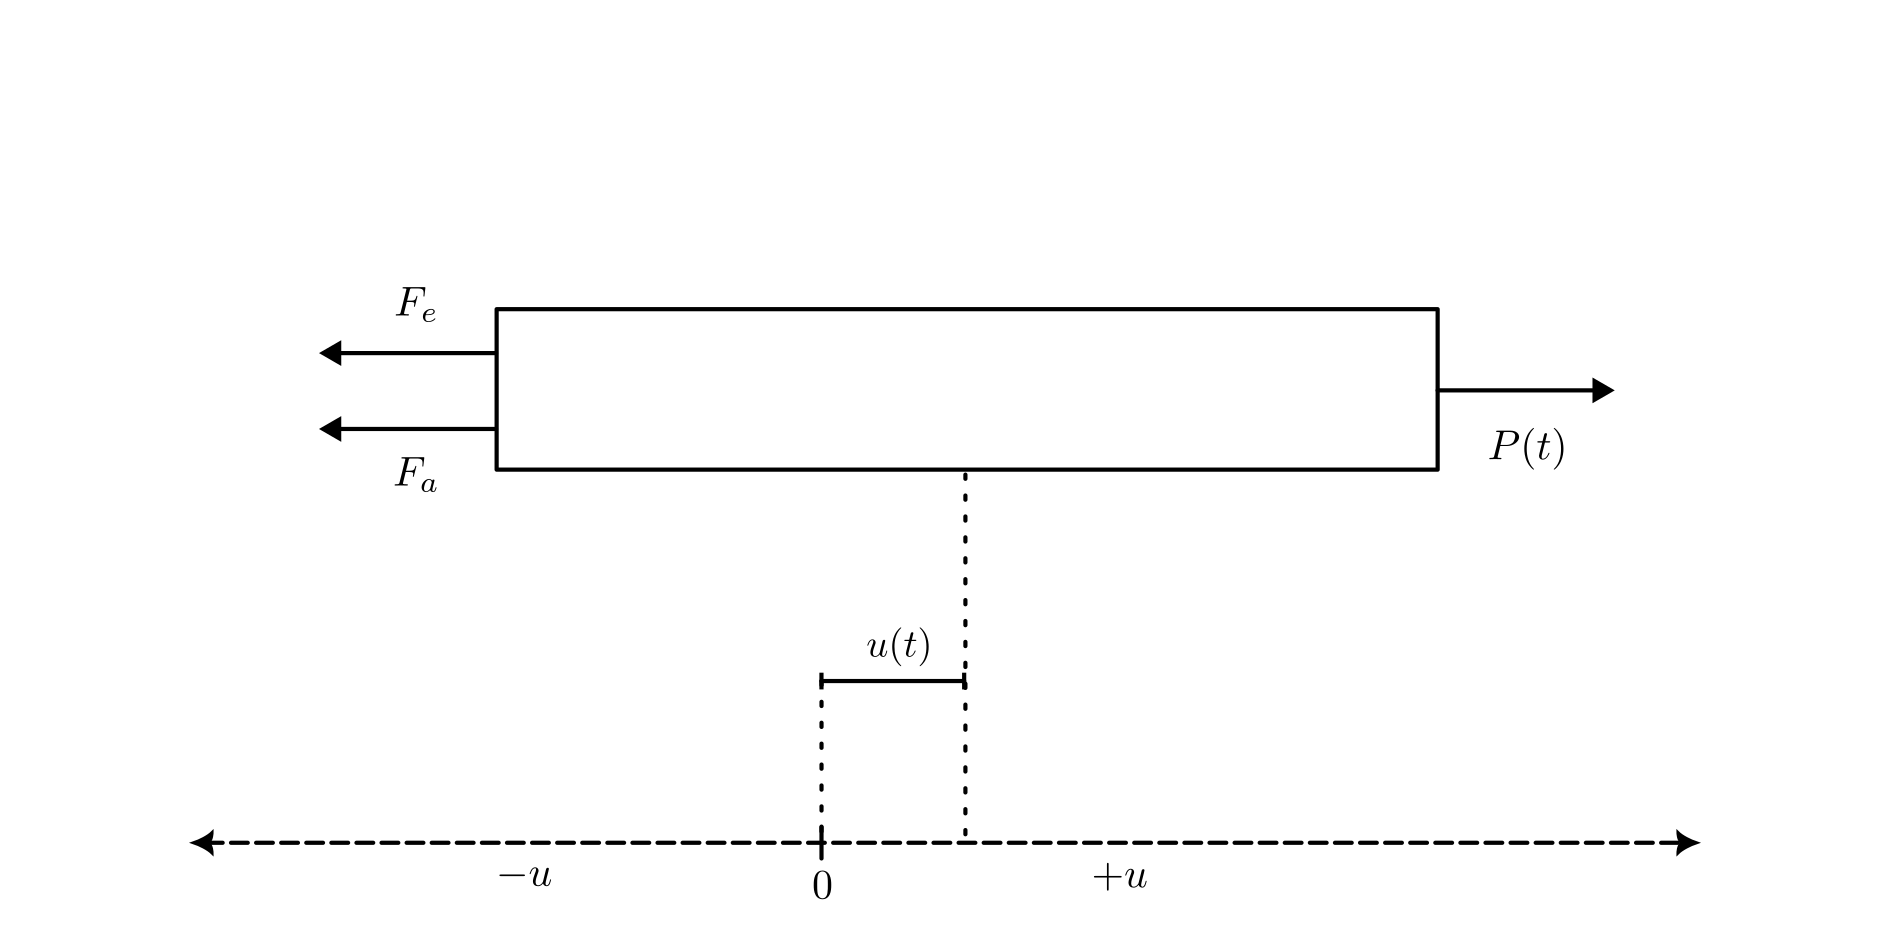
\includegraphics[width=0.8\textwidth]{dcl_1_piso}
    \caption{DCL de la estructura de un piso.}
    \label{fig:1-floor-dcl}
\end{figure}

De este diagrama, podemos identificar tres fuerzas que actúan sobre la estructura. En primer lugar, la ley de Hooke (tomando al sistema como un sistema masa-resorte) implica una fuerza de restauración \(F_e = -ku\). En segundo lugar, está presente una fuerza de amortiguamiento \(F_a = -cv\), la cual tomamos como proporcional a la velocidad horizontal del objeto. Finalmente, está presente la fuerza de excitación externa \(P(t)\). Sumando estas fuerzas y aplicando la segunda ley de Newton a la estructura, obtenemos que se cumple la relación
\begin{equation}\label{eqn:almost}
    -ku - cv + P(t) = ma
.\end{equation}

Recordando que la velocidad \(v\) y la aceleración \(a\) son la primera y segunda derivada de la posición \(u\) respectivamente, reemplazamos \(v\) y \(a\) en \eqref{eqn:almost} y obtenemos
\begin{equation}
    -ku - c\frac{du}{dt} + P(t) = m\frac{d^2u}{dt^2}
.\end{equation}

Reorganizando los términos, nos queda la relación
\begin{equation}\label{eqn:astroscilaciones}
    m\frac{d^2u}{dt^2} + c\frac{du}{dt} + ku = P(t)
.\end{equation}

\subsection{Modelado para una estructura de tres grados de libertad}

Habiendo realizado el modelado para una estructura de un único piso, consideremos ahora una estructura de tres pisos (véase la figura~\ref{fig:3-floor-diagram}). De forma análoga al modelo anterior, consideraremos cada piso como un grado de libertad en la estructura. Entonces, sean las siguientes variables para el \(i\)-ésimo piso:

\begin{itemize}
    \item \(m_i\): masa (en \si{kg}).
    \item \(u_i(t)\): posición horizontal (en \si{m}).
    \item \(v_i(t)\): velocidad horizontal (en \si{m/s}).
    \item \(a_i(t)\): aceleración horizontal (en \si{m/s^2}).
    \item \(c_i\): constante de amortiguamiento viscoso (en \si{kg/s}).
    \item \(k_i\): constante de amortiguamiento viscoso (en \si{kg/s^2}).
    \item \(P_i(t)\): fuerza de excitación (en \si{N}).
\end{itemize}

\begin{figure}[ht!]
    \centering
    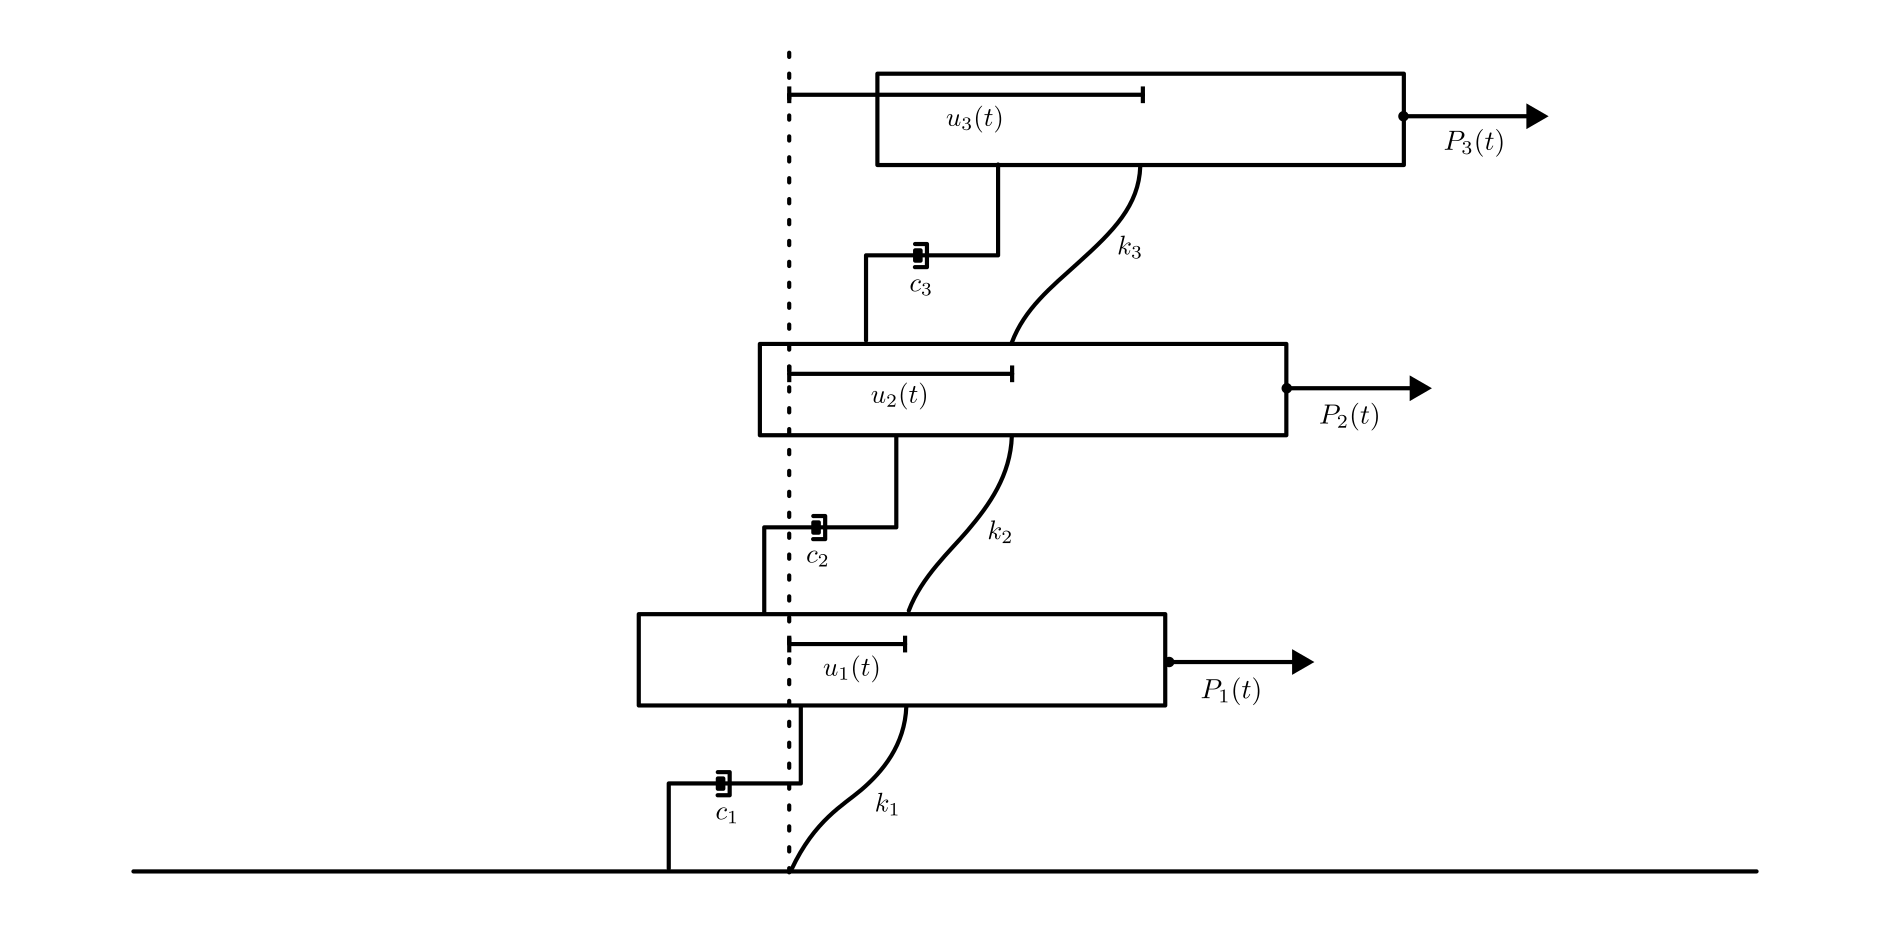
\includegraphics[width=0.9\textwidth]{diagrama_3_pisos}
    \caption{Una estructura de 3 pisos, sus constantes elásticas y de amortiguamiento, y sus fuerzas de excitación externas.}
    \label{fig:3-floor-diagram}
\end{figure}

Podemos notar de la figura~\ref{fig:3-floor-diagram} que, en esta configuración, cada piso interactúa con sus pisos adyacentes por medio de las fuerzas de restauración y amortiguamiento. Por lo tanto, al derivar una expresión similar a \eqref{eqn:astroscilaciones} para el \(i\)-ésimo piso, es necesario considerar dichas interacciones en ese piso particular.

Por lo tanto, haremos un análisis con DCL para cada piso individualmente.

\subsubsection*{Piso 1}

Como muestra el DCL de la figura~\ref{fig:3-floor-dcl-1}, el primer piso de la estructura se ve afectado por fuerzas de restauración y amortiguamiento viscoso con respecto tanto al \textit{suelo} como al \textit{segundo piso}.

\begin{figure}[ht!]
    \centering
    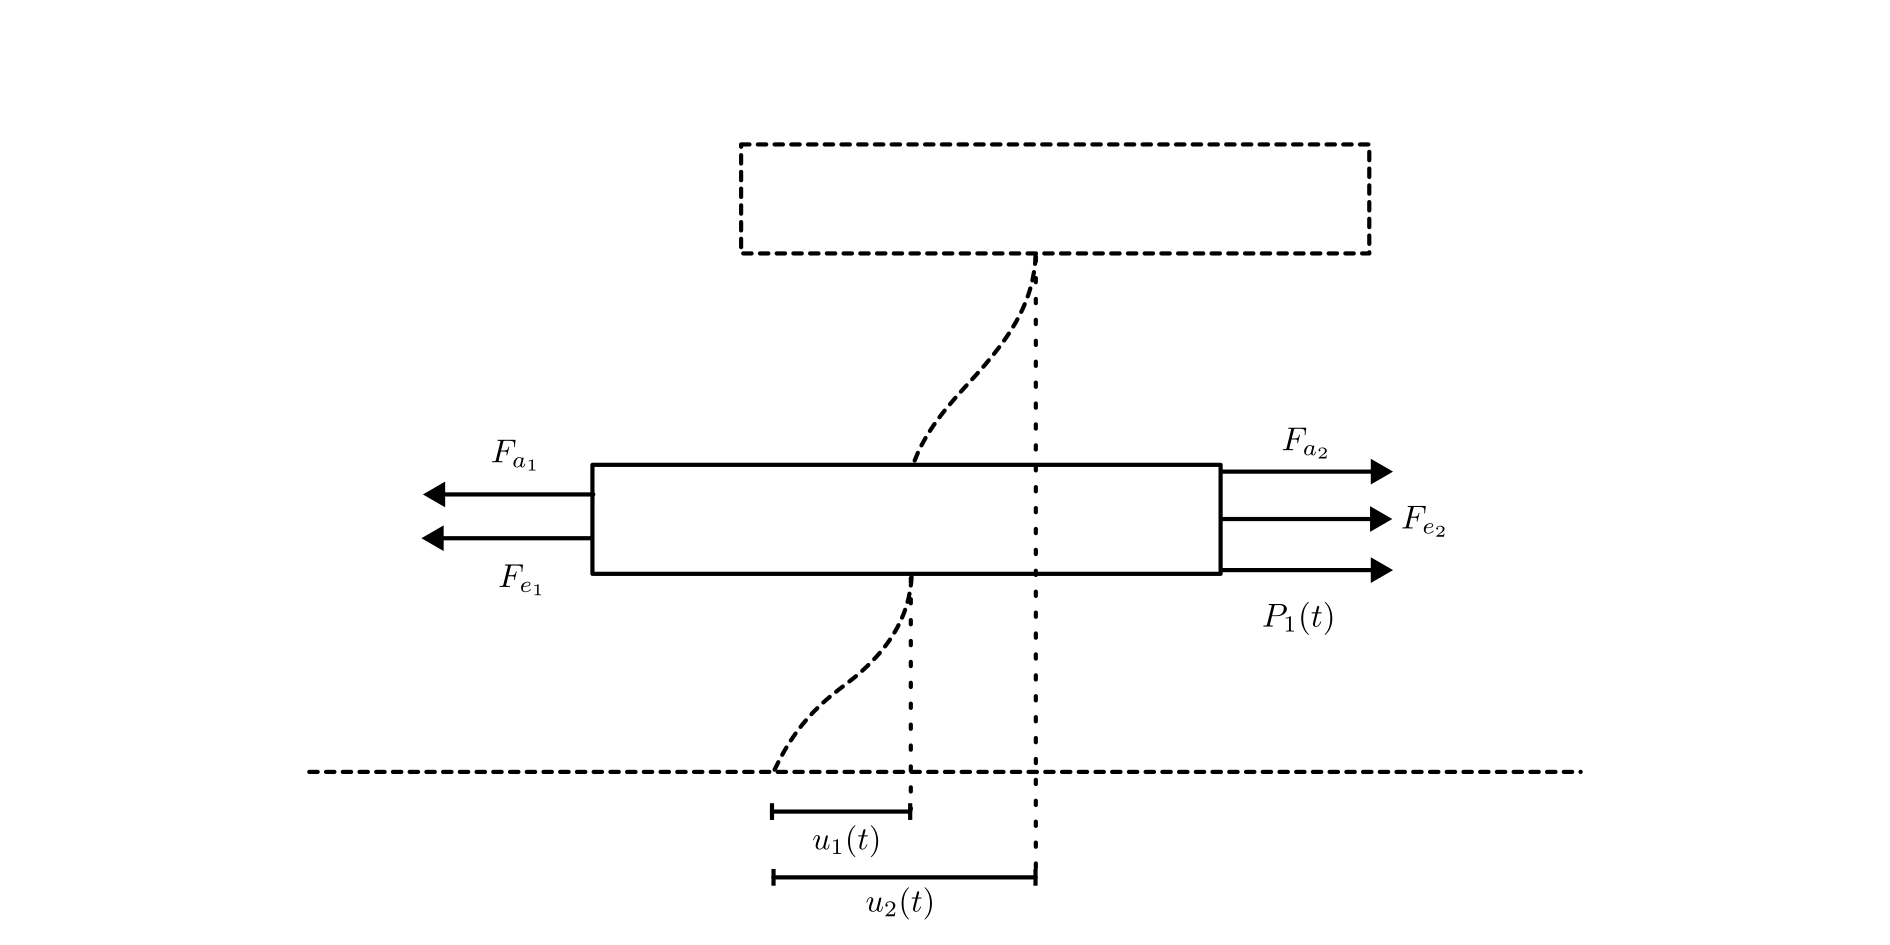
\includegraphics[width=0.8\textwidth]{dcl_3_pisos_1}
    \caption{DCL del primer piso de la estructura.}
    \label{fig:3-floor-dcl-1}
\end{figure}

Nótese que la fuerza elástica ejercida por la interacción con el segundo piso actúa sobre la distancia \(u_1 - u_2\), ya que se trata del desplazamiento del piso 1 \textit{con respecto al piso 2}. Lo mismo aplica para la fuerza de amortiguamiento provocada por el segundo piso.

Con estas consideraciones, deducimos que el primer piso se ve afectado por las fuerzas de restauración
\[
    F_{e_1} = -k_1 u_1, \quad F_{e_2} = -k_2(u_1 - u_2)
,\]
las fuerzas de amortiguamiento viscoso
\[
    F_{a_1} = -c_1 v_1 \quad F_{a_2} = -c_2(v_1 - v_2)
\]
y la fuerza de excitación \(P_1(t)\).

Sumando estas fuerzas y aplicando la segunda ley de Newton para este piso, obtenemos
\[
    -k_1 u_1 - k_2(u_1 - u_2) - c_1 v_1 - c_2(v_1 - v_2) + P_1(t) = m_1 a_1
.\]

Reemplazando \(v_1\) y \(a_1\) por la primera y segunda derivada de \(u_1\) respectivamente y reorganizando los términos, obtenemos
\begin{equation}\label{eqn:floor-1}
    m_1 u_1'' + c_1 u_1' + c_2(u_1' - u_2') + k_1 u_1 + k_2(u_1 - u_2) = P_1(t)
.\end{equation}


\subsubsection*{Piso 2}

La figura  muestra el DCL del segundo piso de la estructura.

\begin{figure}[ht!]
    \centering
    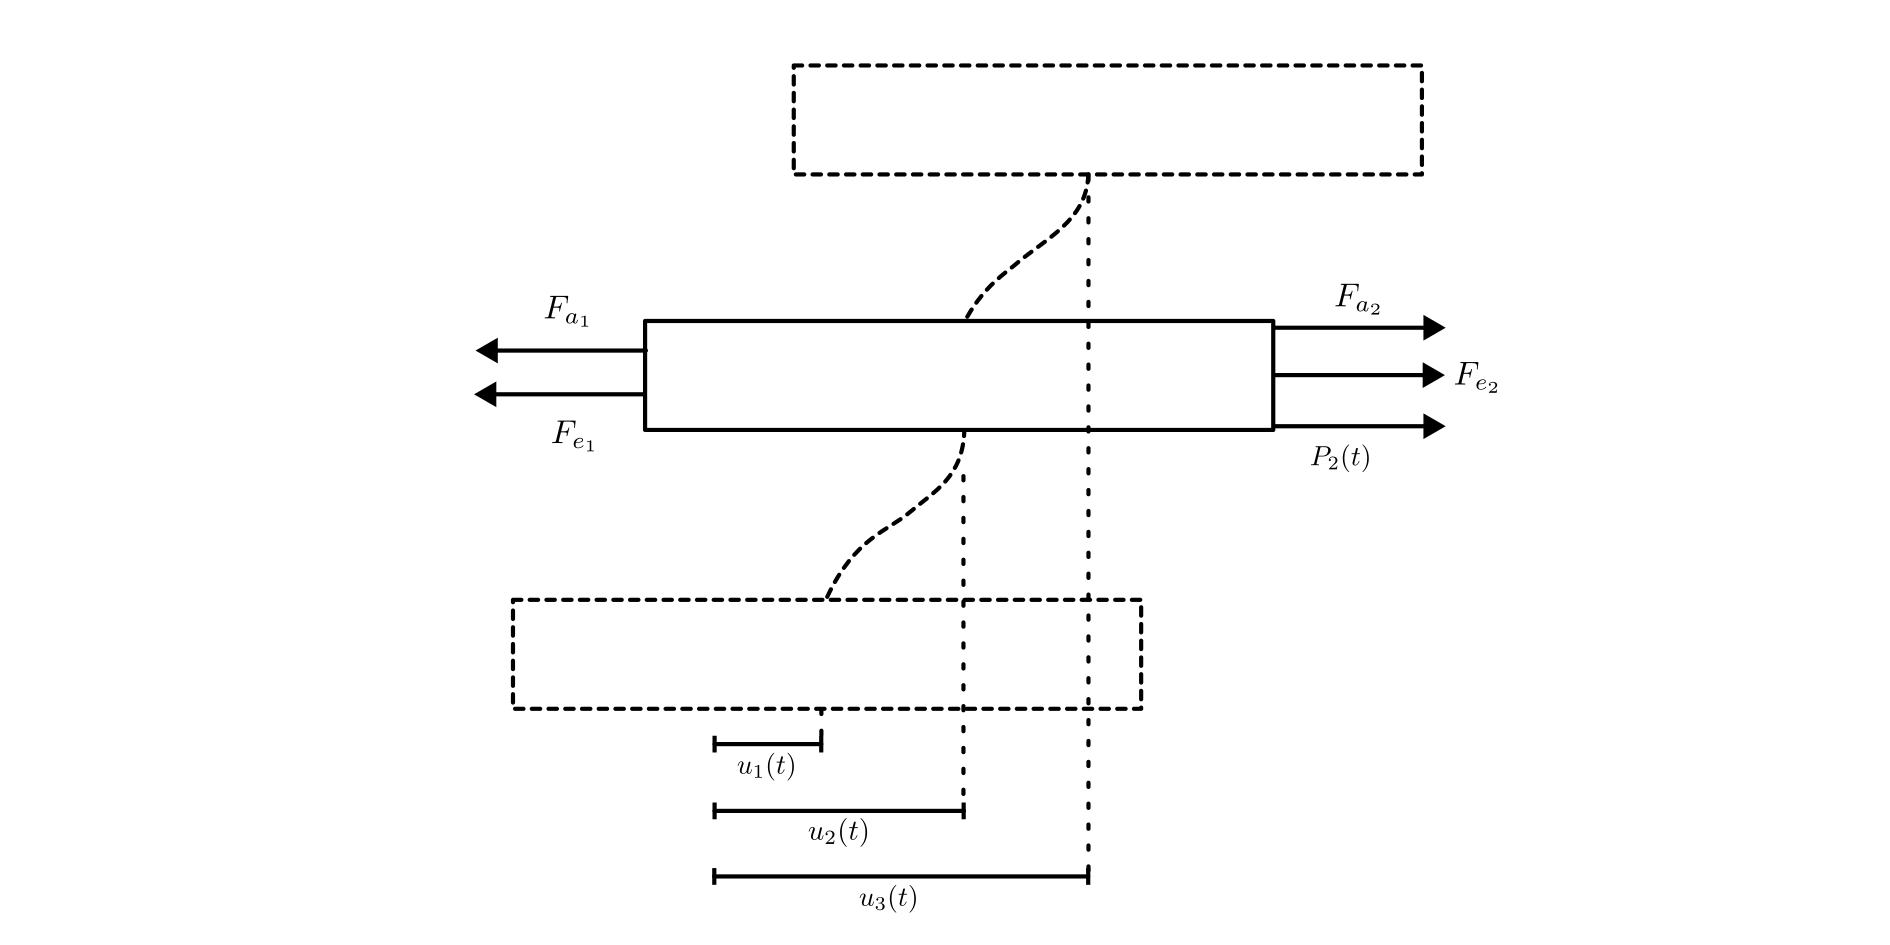
\includegraphics[width=0.8\textwidth]{dcl_3_pisos_2}
    \caption{DCL del segundo piso de la estructura.}
    \label{fig:3-floor-dcl-2}
\end{figure}

De igual manera al piso 1, debemos considerar los desplazamientos respecto a los cuales se aplican las fuerzas de restauración y amortiguamiento. Para este caso, estas fuerzas ocurren sobre los desplazamientos relativos \(u_2 - u_1\) y \(u_2 - u_3\) (es decir, del piso 2 con respecto al piso 1 y al piso 3, respectivamente). Este piso se ve afectado por las fuerzas de restauración
\[
    F_{e_1} = -k_2(u_2 - u_1), \quad F_{e_2} = -k_3(u_2 - u_3)
,\]
las fuerzas de amortiguamiento viscoso
\[
    F_{a_1} = -c_2(v_2 - v_1) \quad F_{a_2} = -c_3(v_2 - v_3)
\]
y la fuerza de excitación \(P_2(t)\).

Sumando estas fuerzas y aplicando la segunda ley de Newton, obtenemos
\[
    -k_2(u_2 - u_1) - k_3(u_2 - u_3) - c_2(v_2 - v_1) - c_3(v_2 - v_3) + P_2(t) = m_2 a_2
.\]

Reemplazando velocidades y aceleraciones por las derivadas de \(u_2\) y reordenando, esto se convierte en
\begin{equation}\label{eqn:floor-2}
    m_2 u_2'' + c_2(u_2' - u_1') + c_3(u_2' - u_3') + k_2(u_2 - u_1) + k_3(u_2 - u_3) = P_2(t)
.\end{equation}


\subsubsection*{Piso 3}

La figura  muestra el DCL del tercer piso de la estructura.

\begin{figure}[ht!]
    \centering
    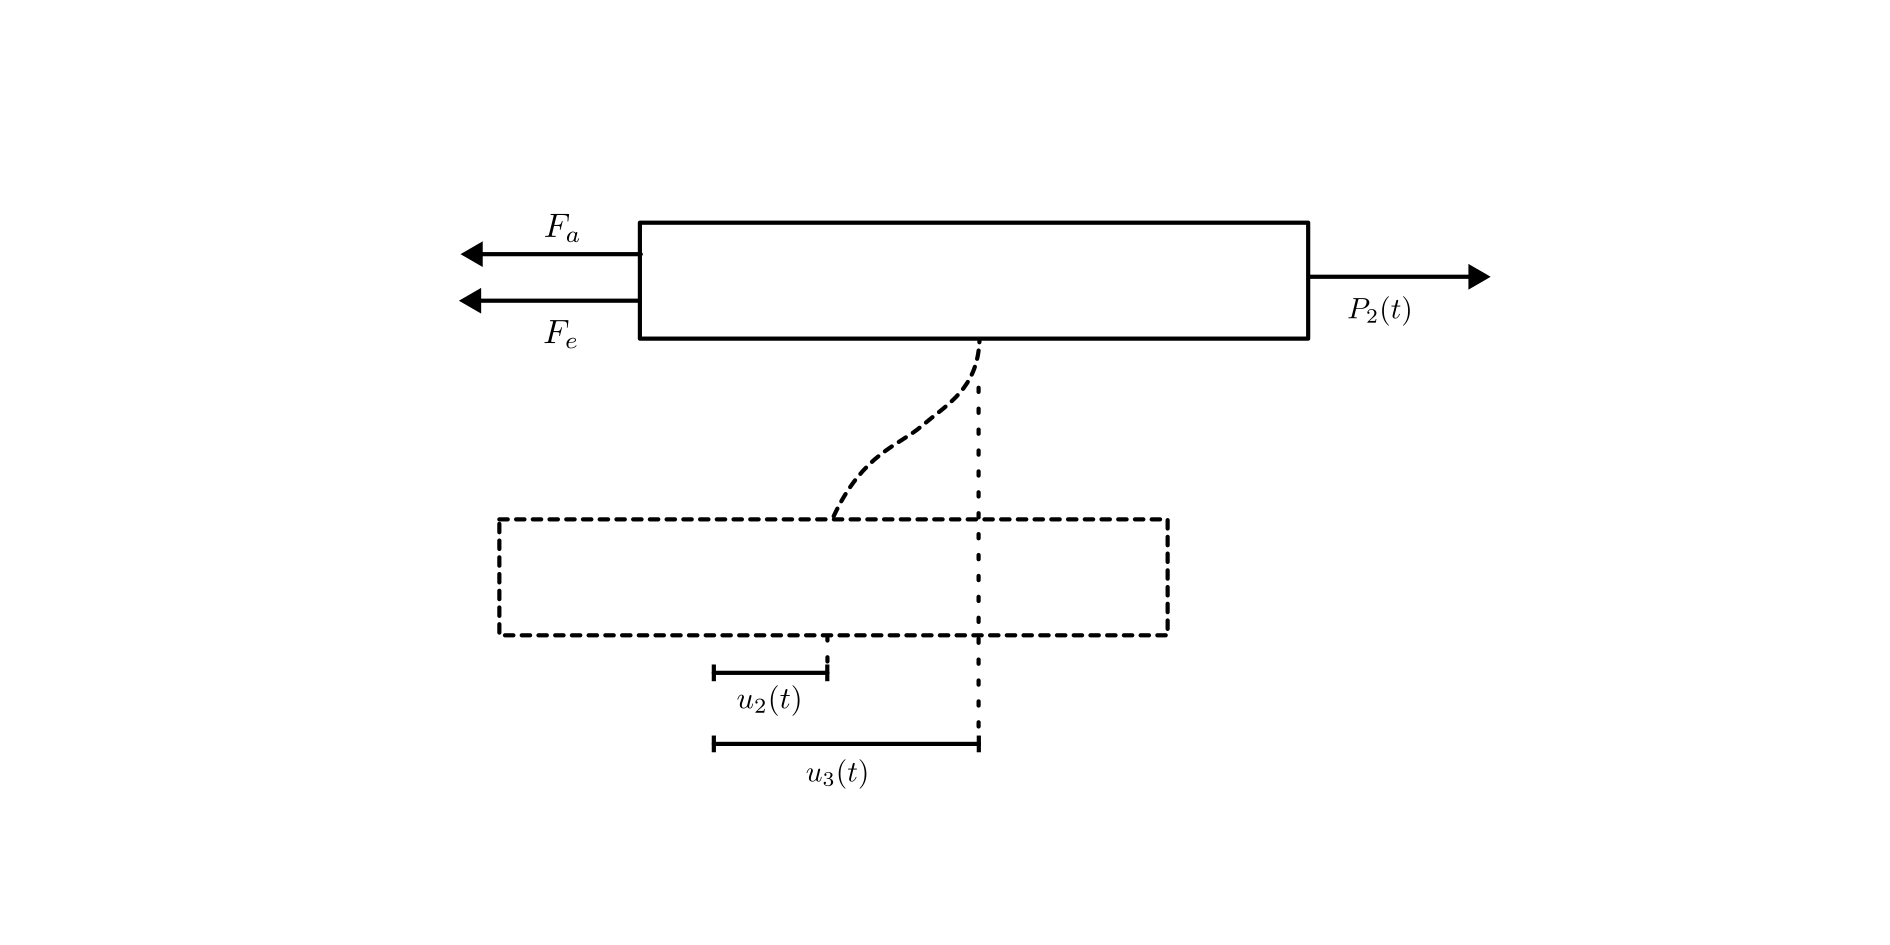
\includegraphics[width=0.8\textwidth]{dcl_3_pisos_3}
    \caption{DCL del tercer piso de la estructura.}
    \label{fig:3-floor-dcl-3}
\end{figure}


Podemos observar que el tercer piso solo se ve afectado por las fuerzas de restauración y amortiguamiento de su conexión al piso 2 porque ya no tiene otro piso por encima. El único desplazamiento relativo con respecto al cual se aplican las fuerzas de restauración y amortiguamiento es \(u_3 - u_3\) (es decir, su posición con respecto al piso 2).

Por lo tanto, este piso se ve afectado por las fuerzas de restauración y amortiguamiento viscoso
\[
    F_e = -k_3(u_3 - u_2), \quad F_a = -c_3(v_3 - v_2)
,\]
además de la fuerza de excitación \(P_3(t)\).

Sumando estas fuerzas y aplicando la segunda ley de Newton, obtenemos la ecuación
\[
    -k_3(u_3 - u_2) - c_3(v_3 - v_2) + P_3(t) = m_3 a_3
.\]

Reemplazando velocidades y aceleraciones por las derivadas de \(u_3\) y reordenando términos, obtenemos
\begin{equation}\label{eqn:floor-3}
    m_3 u_3'' + c_3(u_3' - u_2') + k_3(u_3 - u_2) = P_3(t)
.\end{equation}


\subsubsection*{Modelo final}

Juntando \eqref{eqn:floor-1}, \eqref{eqn:floor-2} y \eqref{eqn:floor-3}, obtenemos el sistema

\begin{align*}
    m_1 u_1'' + c_1 u_1' + c_2(u_1' - u_2') + k_1 u_1 + k_2(u_1 - u_2) &= P_1(t) \\
    m_2 u_2'' + c_2(u_2' - u_1') + c_3(u_2' - u_3') + k_2(u_2 - u_1) + k_3(u_2 - u_3) &= P_2(t) \\
    m_3 u_3'' + k_3(u_3 - u_2) + c_3(u_3' - u_2') &= P_3(t)
,\end{align*}
el cual se puede expresar en forma matricial como
\begin{equation}\label{eqn:matrix-form}
    M\mathbf{u}'' + C\mathbf{u}' + K\mathbf{u} = \mathbf{P}(t)
,\end{equation}
donde
\begin{equation}
    \mathbf{u}(t) = \begin{bmatrix} u_1(t) \\ u_2(t) \\ u_3(t) \end{bmatrix},
    \quad
    M = \begin{bmatrix}
        m_1 & 0 & 0 \\
        0 & m_2 & 0 \\
        0 & 0 & m_3
    \end{bmatrix},
    \quad
    \mathbf{P}(t) = \begin{bmatrix} P_1(t) \\ P_2(t) \\ P_3(t) \end{bmatrix}
\end{equation}
y las matrices de constantes de elasticidad y amortiguamiento viscoso, respectivamente, son
\begin{equation}
    K = \begin{bmatrix}
        k_1 + k_2 & -k_2 & 0 \\
        -k_2 & k_2 + k_3 & -k_3 \\
        0 & -k_3 & k_3
    \end{bmatrix},
    \quad
    C = \begin{bmatrix}
        c_1 + c_2 & -c_2 & 0 \\
        -c_2 & c_2 + c_3 & -c_3 \\
        0 & -c_3 & c_3
    \end{bmatrix}
.\end{equation}

Este es un sistema de 3 ecuaciones diferenciales lineales de segundo orden, y modela las vibraciones mecánicas de una estructura de 3 pisos. Considerar \eqref{eqn:astroscilaciones} con \(\mathbf{P}(t) = \mathbf{0}\) se puede utilizar para hallar la \textit{frecuencia natural} de la estructura \citep{rendon}.

\subsection{Para una estructura de múltiples grados de libertad}

No resulta difícil extender el modelo de 3 pisos a una cantidad arbitraria de pisos. En esencia, el procedimiento consistirá en modelar el primer piso, un piso intermedio cualquiera, y el último piso.

Consideremos una estructura de \(n\) pisos para \(n \geq 3\), considerando las mismas variables usadas para el \(i\)-ésimo piso del modelo de 3 pisos. Nuevamente, consideraremos cada piso de la estructura como un grado de libertad en sentido horizontal.

De manera similar al modelo de 3 pisos, vamos a modelar las ecuaciones para el primer piso, un piso intermedio cualquiera (entre el primero y el último), y el último piso.

\subsubsection*{Piso 1}

El procedimiento para modelar este piso es exactamente el mismo que el del primer piso del modelo anterior, y tiene un DCL idéntico a la figura~\ref{fig:3-floor-dcl-1}. Realizando el mismo procedimiento exacto que en aquel, obtenemos una ecuación igual a \eqref{eqn:floor-1}:
\begin{equation}\label{eqn:final-floor-1}
    m_1 u_1'' + c_1 u_1' + c_2(u_1' - u_2') + k_1 u_1 + k_2(u_1 - u_2) = P_1(t)
.\end{equation}

\subsubsection*{Piso intermedio}

El proceso para estos pisos es exactamente igual al del segundo piso del modelo de estructura de 3 pisos, pero tomando al piso 1 de ese modelo como el piso \(i - 1\), y al piso 3 de ese modelo como el piso \(i + 1\). Por completitud, de todas formas incluimos de forma breve la derivación de la ecuación para estos pisos intermedios.

Consideremos ahora un \(i\)-ésimo piso para \(1 < i < n\), cuyo DCL se muestra en la figura~\ref{fig:n-floor-dcl-mid}.

\begin{figure}[ht!]
    \centering
    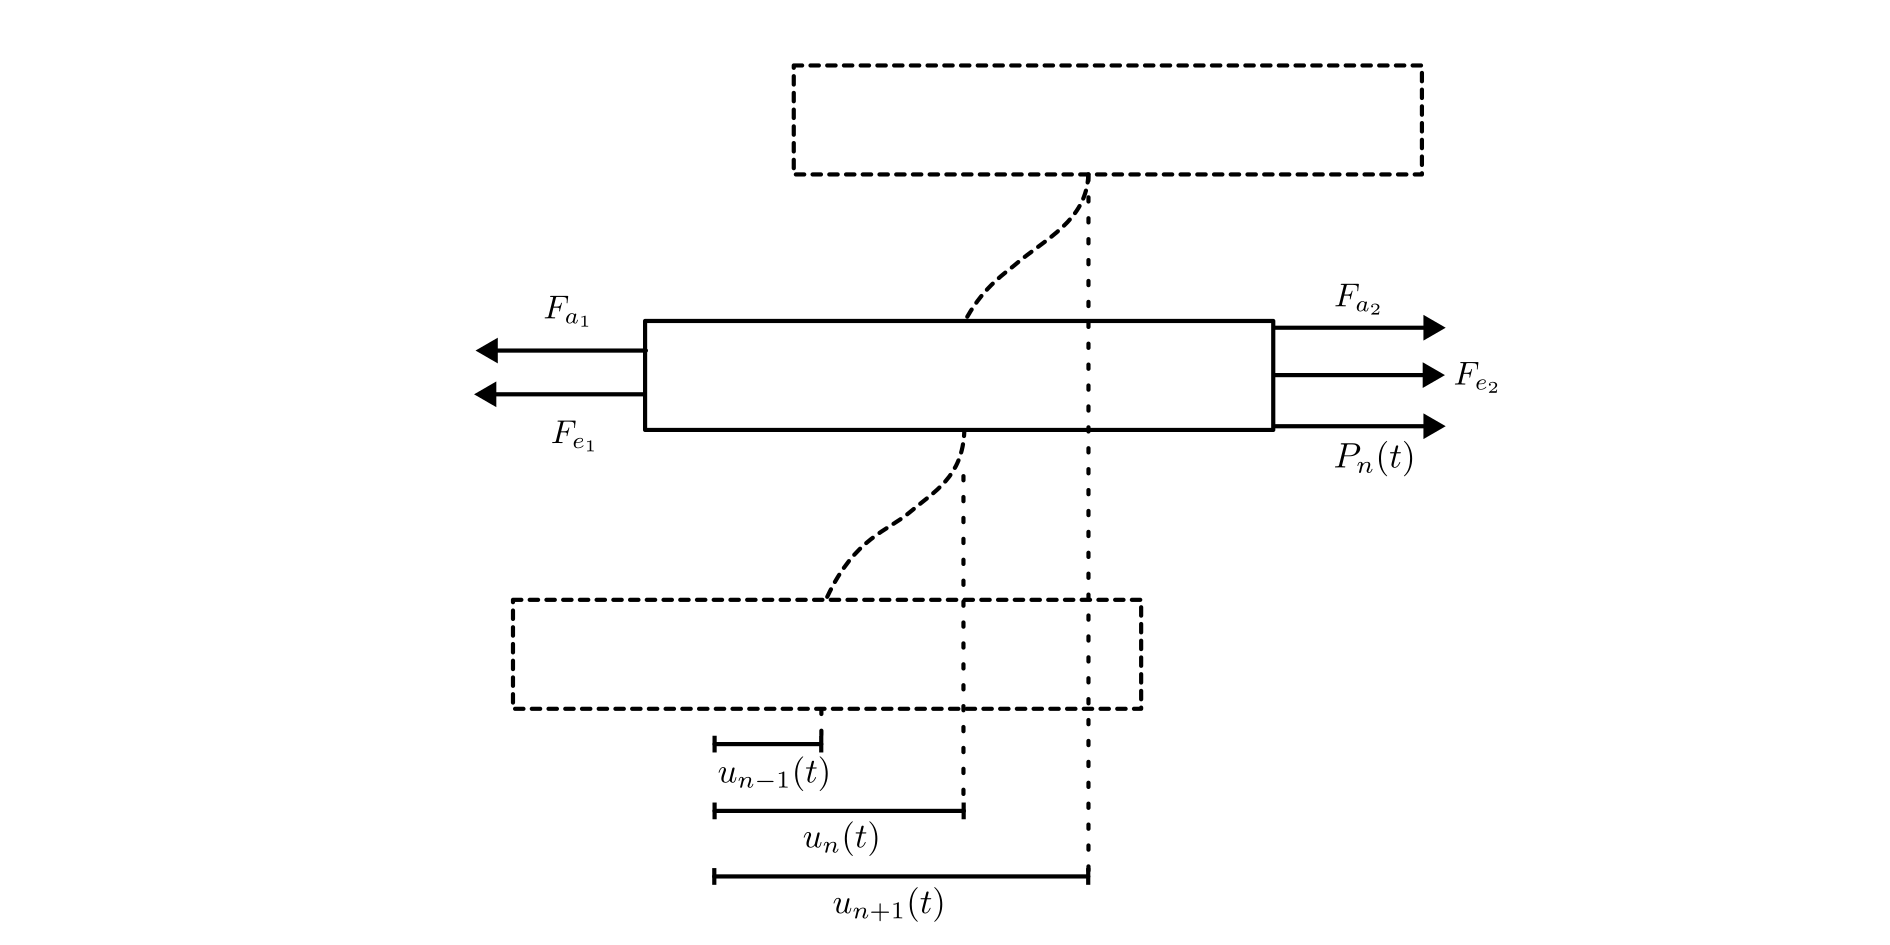
\includegraphics[width=0.8\textwidth]{dcl_n_pisos_mid}
    \caption{DCL de un \(i\)-ésimo piso de la estructura.}
    \label{fig:n-floor-dcl-mid}
\end{figure}

Este piso se ve afectado por fuerzas de restauración y amortiguamiento viscoso tanto por los pisos \(i - 1\) y \(i + 1\). Por lo tanto, las fuerzas de restauración que afectan a este piso son
\[
    F_{e_1} = -k_i(u_i - u_{i-1}), \quad F_{e_2} = -k_{i+1}(u_i - u_{i+1})
,\]
las fuerzas de amortiguamiento viscoso que lo afectan son
\[
    F_{a_1} = -c_i(v_i - v_{i-1}) \quad F_{a_2} = -c_{i+1}(v_i - v_{i+1})
,\]
y además se ve afectado por la fuerza de excitación \(P_i(t)\).

Sumando estas fuerzas y aplicando segunda ley de Newton, obtenemos
\[
    -k_i(u_i - u_{i-1}) - k_{i+1}(u_i - u_{i+1}) - c_i(v_i - v_{i-1}) - c_{i+1}(v_i - v_{i+1}) + P_i(t) = m_i a_i
.\]
Reemplazando velocidades y aceleraciones por las derivadas de \(u_i\) y reordenando, obtenemos que el \(i\)-ésimo piso se modela mediante la ecuación
\begin{equation}\label{eqn:final-floor-mid}
    m_i u_i'' + c_i(u_i' - u_{i-1}') + c_{i+1}(u_i' - u_{i+1}') + k_i(u_i - u_{i-1}) + k_{i+1}(u_i - u_{i+1}) = P_i(t)
.\end{equation}

\subsubsection*{Último piso}

Consideremos ahora el \(n\)-ésimo piso, cuyo DCL es idéntico al de la figura~\ref{fig:3-floor-dcl-3}, pero tomando al piso 3 como el piso \(n\) y al piso 2 como el piso \(n - 1\). Nuevamente, el procedimiento para modelar este piso es exactamente el mismo que para el piso 3 de la estructura de 3 pisos. Un tratamiento esencialmente idéntico al que realizamos para ese caso anterior nos otorga una expresión idéntica a \eqref{eqn:floor-3}, pero reemplazando al piso 3 por el piso \(n\) y al piso 2 por el piso \(n - 1\):
\begin{equation}\label{eqn:final-floor-last}
    m_n u_n'' + c_n(u_n' - u_{n-1}') + k_n(u_n - u_{n-1}) = P_n(t)
.\end{equation}


\subsubsection*{Modelo final}

Juntando las ecuaciones \eqref{eqn:final-floor-1}, \eqref{eqn:final-floor-mid} y \eqref{eqn:final-floor-last}, obtenemos el sistema de ecuaciones
\begin{align*}
    m_1 u_1'' + c_1 u_1' + c_2(u_1' - u_2') + k_1 u_1 + k_2(u_1 - u_2) &= P_1(t) \\
    m_2 u_2'' + c_1(u_2' - u_1') + c_2(u_2' - u_3') + k_2(u_2 - u_1) + k_3(u_2 - u_3) &= P_2(t) \\
    m_3 u_3'' + c_2(u_3' - u_2') + c_3(u_3' - u_4') + k_3(u_3 - u_2) + k_4(u_3 - u_4) &= P_3(t) \\
    \vdots \qquad &= \quad \vdots \\
    m_{n-1} u_{n-1}'' + c_{n-1}(u_{n-1}' - u_{n-2}') + c_n(u_{n-1}' - u_n') + k_{n-1}(u_{n-1} - u_{n-2}) + k_n(u_{n-1} - u_n) &= P_{n-1}(t) \\
    m_n u_n'' + c_n(u_n' - u_{n-1}') + k_n(u_n - u_{n-1}) &= P_n(t)
.\end{align*}

Este sistema de \(n\) ecuaciones se puede representar en forma matricial como
\begin{equation}\label{eqn:final-matrix-form}
    M\mathbf{u}'' + C\mathbf{u}' + K\mathbf{u} = \mathbf{P}(t)
,\end{equation}
donde
\begin{equation}
    \mathbf{u}(t) = \begin{bmatrix} u_1(t) \\ u_2(t) \\ \vdots \\ u_n(t) \end{bmatrix},
    \quad
    M = \begin{bmatrix}
        m_1 & 0 & \cdots & 0 \\
        0 & m_2 & \cdots & 0 \\
        \vdots & \vdots & \ddots & \vdots \\
        0 & 0 & \cdots & m_n
    \end{bmatrix},
    \quad
    \mathbf{P}(t) = \begin{bmatrix} P_1(t) \\ P_2(t) \\ \vdots \\ P_n(t) \end{bmatrix}
\end{equation}
y las matrices de constantes de elasticidad y amortiguamiento viscoso, respectivamente, son
\begin{equation}
    K = \begin{bmatrix}
        k_1 + k_2 & -k_2 & 0 & 0 & \cdots & 0 \\
        -k_2 & k_2 + k_3 & -k_3 & 0 & \cdots & 0 \\
        0 & -k_3 & k_3 + k_4 & -k_4 & \cdots & 0 \\
        \vdots & \vdots & \ddots & \ddots & \ddots & \vdots \\
        0 & 0 & \cdots & -k_{n-1} & k_{n-1} + k_n & -k_n \\
        0 & 0 & \cdots & 0 & -k_{n} & k_n
    \end{bmatrix}
\end{equation}
y
\begin{equation}
    C = \begin{bmatrix}
        c_1 + c_2 & -c_2 & 0 & 0 & \cdots & 0 \\
        -c_2 & c_2 + c_3 & -c_3 & 0 & \cdots & 0 \\
        0 & -c_3 & c_3 + c_4 & -c_4 & \cdots & 0 \\
        \vdots & \vdots & \ddots & \ddots & \ddots & \vdots \\
        0 & 0 & \cdots & -c_{n-1} & c_{n-1} + c_n & -c_n \\
        0 & 0 & \cdots & 0 & -c_{n} & c_n
    \end{bmatrix}
.\end{equation}

Este es un sistema de \(n\) ecuaciones diferenciales de segundo orden, y es el sistema que modela las oscilaciones de una estructura de \(n\) pisos. Al igual que en el modelo de 3 pisos, considerar \eqref{eqn:final-matrix-form} con \(\mathbf{P}(t) = \mathbf{0}\) se puede utilizar para hallar la frecuencia natural de la estructura \citep{rendon}.

\section{Análisis previo del problema}

Antes de resolver el sistema de ecuaciones diferenciales propuesto, presentamos aquí un repaso de todas las variables y parámetros involucrados, considerando una estructura de \(n\) pisos.

\begin{enumerate}
    \item \textbf{Posiciones (\(u_1(t), u_2(t), \ldots, u_n(t)\)):} Son las posiciones horizontales (en metros) de cada piso, respectivamente. Como recalcamos anteriormente, en este informe se considera a la derecha como el eje positivo. Además, se consideran en función del tiempo.

    \item \textbf{Masas (\(m_1, m_2, \ldots, m_n\)):} Son las masas (en \(\si{kg}\)) de cada piso, respectivamente. Naturalmente, todas las masas deben ser números positivos.

        En contexto del modelo, las masas se ven involucradas en la fuerza requerida para afectar el movimiento de un piso particular. Esto se demuestra por la segunda ley de Newton, \(\sum F_i = ma\).

    \item \textbf{Constantes de amortiguamiento (\(c_1, c_2, \ldots, c_n\)):} Son los coeficientes de amortiguamiento (en \(kg/s\)) de cada piso, respectivamente. Representan la resistencia de cada piso a permanecer en movimiento debido a factores del medio, como la resistencia del aire. Como estamos tomando la ecuación de amortiguamiento \(F_a = -cv\) con el signo negativo ya incluido, estas constantes deben ser no-negativas.

        En contexto del modelo, las constantes de amortiguamiento funcionan como la medida de qué tan rápido se ''estabilizaría`` un piso dado al estar oscilando. Si todas las constantes de amortiguamiento fuesen nulas, entonces un movimiento oscilatorio en la estructura permanecería para siempre aunque las fuerzas externas cesaran.

    \item \textbf{Constantes elásticas \(k_1, k_2, \ldots, k_n\)}: Son los coeficientes elásticos (en \(\si{kg/s^2}\)) de cada piso, respectivamente. Más precisamente, se pueden interpretar como el coeficiente elástico de la \textit{unión} de un piso con el que tiene por debajo. De la misma forma que las constantes de amortiguamiento, este informe considera la ley de Hooke \(F_e = -kx\) con el signo negativo incluido, así que las constantes elásticas toman valores no-negativos.

    \item \textbf{Fuerzas externas (\(P_1(t), P_2(t), \ldots, P_n(t)\)):} Son las fuerzas externas (en \(\si{N}\)) siendo aplicadas a cada piso en función del tiempo. Más precisamente, actúan en el eje horizontal.

        En contexto del modelo, las fuerzas externas son las que generan el comportamiento (usualmente) oscilatorio de los pisos de la estructura. En general, a mayor magnitud tengan estas fuerzas, mayores se esperaría que fuesen los desplazamientos de los pisos.

        Además, la forma de estas fuerzas también determina el comportamiento del desplazamiento de los pisos. Si algún \(P_i(t)\) toma como valor una función sinusoidal, se esperaría que los pisos oscilen indefinidamente a la misma frecuencia que la fuerza. Si \(\mathbf{P}(t)\) contuviese impulsos breves de fuerza (con forma de campana gaussiana, por ejemplo), se esperaría que los pisos oscilen, pero que la amplitud de dicha oscilación progresivamente vuelva a 0.

\end{enumerate}

Como se ha mostrado en la sección anterior, estas variables y parámetros se agrupan en matrices para presentar las ecuaciones de forma más condensada.

\section{Método de solución}

Consideraremos una estructura de \(n\) pisos, la cual se puede modelar mediante \eqref{eqn:final-matrix-form}. Además, consideraremos que la estructura parte del reposo y de la posición de equilibrio. Esto nos aporta las condiciones iniciales \(\mathbf{u}(0) = \mathbf{0}\) y \(\mathbf{u}'(0) = \mathbf{0}\).

\subsection{Intento mediante eigenvalores y eigenvectores}

Podemos considerar el problema reducido de las ecuaciones para una estructura de \(n = 2\) pisos bajo los siguientes parámetros simplificados:
\begin{gather}
	m_1 = m_2 = m \\
	c_2 = 0, \, c_1 = c \\
	k_1 = k_2 = k \\
	P_1(t) = A\sin(\omega t), \, P_2(t) = 0
.\end{gather}

La ecuación sería la siguiente:
\[
	\begin{bmatrix}
    	m & 0 \\
    	0 & m
	\end{bmatrix} \begin{bmatrix} u_1'' \\ u_2'' \end{bmatrix}
	+ \begin{bmatrix}
    	c & 0 \\
    	0 & 0
	\end{bmatrix} \begin{bmatrix} u_1' \\ u_2' \end{bmatrix}
	+ \begin{bmatrix}
    	2k & -k \\
    	-k & k
	\end{bmatrix} \begin{bmatrix} u_1 \\ u_2 \end{bmatrix}
	= \begin{bmatrix} A\sin(\omega t) \\ 0 \end{bmatrix}
,\]

la cual se puede expresar como el sistema
\[
	\begin{cases}
    	mu_1'' + cu_1' + 2ku_1 - ku_2 = A\sin(\omega t) \\
    	mu_2'' - ku_1 + ku_2 = 0
	.\end{cases}
\]

Empezamos realizando un cambio de variable para poder construir un sistema de primer orden:
\[
	\begin{cases}
    	u_1'=v_1 \\
    	u_2'=v_2.
	\end{cases}
\]

El nuevo sistema toma la siguiente forma:
\[
	\begin{cases}
    	u_1'=v_1 \\
    	u_2'=v_2 \\
    	mv_1' + cv_1 + 2ku_1 - ku_2 = A\sin(\omega t) \\
    	mv_2' - ku_1 + ku_2 = 0.
	\end{cases}
\]

Despejado las derivadas a un lado de la ecuación, obtenemos
\[
	\begin{cases}
    	u_1' = v_1 \\
    	u_2' = v_2 \\
    	v_1' = - \frac{2k}{m}u_1 + \frac{k}{m}u_2 - \frac{c}{m}v_1 + \frac{A}{m}\sin(\omega t) \\
    	v_2' = \frac{k}{m}u_1 - \frac{k}{m}u_2.
	\end{cases}
.\]

Expresando el sistema en su forma matricial \(X' = AX\) se obtiene la expresión
\[
    \begin{bmatrix} u_1' \\ u_2' \\ v_1' \\ v_2' \end{bmatrix} =
    \begin{bmatrix}
        0 & 0 & 1 & 0 \\
   	0 & 0 & 0 & 1 \\
    -\frac{2k}{m} & \frac{k}{m} & -\frac{c}{m} & 0 \\
    \frac{k}{m} & -\frac{k}{m} & 0 & 0
    \end{bmatrix} \begin{bmatrix} u_1 \\ u_2 \\ v_1 \\ v_2 \end{bmatrix}
    + \begin{bmatrix} 0 \\ 0 \\ \frac{A}{m}\sin(\omega t) \\ 0 \end{bmatrix}
.\]

Para resolver el sistema lineal, podemos usar el método de eigenvalores y eigenvectores. Para esto, primero resolvemos el sistema homogéneo. Empezamos hallando los eigenvalores mediante la ecuación característica \(\det(A-\lambda I) = 0\):
\[
	p(\lambda ) = \begin{vmatrix}
        -\lambda & 0 & 1 & 0 \\
        0 & -\lambda & 0 & 1 \\
        -\frac{2k}{m} & \frac{k}{m} & -\frac{c}{m}-\lambda & 0 \\
        \frac{k}{m} & -\frac{k}{m} & 0 & -\lambda
   \end{vmatrix}
   = \lambda^4 + \frac{c}{m}\lambda^3 + \frac{3k}{m}\lambda^2 + \frac{ck}{m^2}\lambda + \frac{k^2}{m^2}
   = 0
.\]

Aunque tenemos una ecuación de grado 4, esta se puede resolver con métodos computacionales.

\subsection{Usando métodos numéricos}

Para resolver este sistema con las condiciones iniciales dadas, utilizaremos el método de Runge-Kutta de orden 4 (RK4), el cual se detalla en el marco teórico del informe. Sin embargo, para ello será necesario llevar \eqref{eqn:final-matrix-form} a la forma
\[
    \mathbf{x}' = \mathbf{f}(t, \mathbf{x})
.\]

Para ello, podemos definir \(\mathbf{v} = \mathbf{u}'\), lo cual transforma \eqref{eqn:final-matrix-form} (un sistema de \(n\) ecuaciones) en el siguiente sistema de \textit{primer orden} de \(2n\) ecuaciones:

\[
    \begin{cases}
        \mathbf{v} = \mathbf{u}' \\
        M\mathbf{v}' + C\mathbf{v} + K\mathbf{u} = \mathbf{P}(t)
    .\end{cases}
\]

Nótese que cada una de estas ecuaciones matriciales aporta \(n\) ecuaciones al sistema.

Para aplicar el método de RK4 a este sistema, lo colocaremos en la forma
\begin{equation}\label{eqn:substituted-system}
    \begin{cases}
        \mathbf{u}' = \mathbf{v} \\
        \mathbf{v}' = M^{-1}(-C\mathbf{v} - K\mathbf{u} + \mathbf{P}(t))
    .\end{cases}
\end{equation}

Nótese también que \(M^{-1}\) siempre existe (y es trivial) puesto que \(M\) es una matriz diagonal cuyos elementos en dicha diagonal son todos no-nulos:
\[
    M^{-1} = \begin{bmatrix}
        1/m_1 & 0 & \cdots & 0 \\
        0 & 1/m_2 & \cdots & 0 \\
        \vdots & \vdots & \ddots & \vdots \\
        0 & 0 & \cdots & 1/m_n
    \end{bmatrix}
.\]

Ahora podemos expresar \eqref{eqn:substituted-system} mediante una sola ecuación matricial con \(\mathbf{u}\) y \(\mathbf{v}\) concatenados en un solo vector \(\mathbf{x}\) como
\begin{equation}\label{eqn:rk4-ready}
    \mathbf{x}' = \mathbf{f}(t, \mathbf{x})
,\end{equation}
donde definimos
\[
    \mathbf{x} = \begin{bmatrix} \mathbf{u} \\ \mathbf{v} \end{bmatrix}_{2n \times 1},
    \qquad
    \mathbf{f}(t, \mathbf{x}) = \mathbf{f}\left(t, \begin{bmatrix} \mathbf{u}_{n \times 1} \\ \mathbf{v}_{n \times 1} \end{bmatrix}\right) = \begin{bmatrix}
        \mathbf{v} \\
        M^{-1}(-C\mathbf{v} - K\mathbf{u} + \mathbf{P}(t))
    \end{bmatrix}_{2n \times 1}
.\]

Nótese que las condiciones iniciales que establecimos (\(\mathbf{u}(0) = \mathbf{u}'(0) = \mathbf{v}(0) = \mathbf{0}\)) producen en conjunto la condición \(\mathbf{x}(0) = \mathbf{0}\). Además, trabajaremos RK4 con el tiempo inicial \(t_0 = 0\).

Entonces, el procedimiento que usaremos será el siguiente:

\begin{enumerate}
    \item Definir un tiempo final \(t_s\) y una cantidad \(s\) de pasos.
    \item Calcular el avance por iteración: \(h = \frac{t_s - t_0}{s}\).
    \item Comenzando en \(t_0 = 0, \mathbf{x}_0 = \mathbf{0}\), iterar \(s\) veces el método de RK4 de la siguiente manera:
        \begin{enumerate}

            \item Calcular, en orden, los siguientes vectores:
                \begin{align*}
                    \mathbf{k}_1 &= \mathbf{f}(t_i, \mathbf{x}_i) \\
                    \mathbf{k}_2 &= \mathbf{f}(t_i + \frac{h}{2}, \mathbf{x}_i + \frac{h}{2}\mathbf{k}_1) \\
                    \mathbf{k}_3 &= \mathbf{f}(t_i + \frac{h}{2}, \mathbf{x}_i + \frac{h}{2}\mathbf{k}_2) \\
                    \mathbf{k}_4 &= \mathbf{f}(t_i + h, \mathbf{x}_i + h\mathbf{k}_3)
                .\end{align*}

            \item Calcular la siguiente iteración de \(\mathbf{x}\) como
                \[
                    \mathbf{x}_{i+1} = \mathbf{x}_i + \frac{h}{6}(\mathbf{k}_1 + 2\mathbf{k}_2 + 2\mathbf{k}_3 + \mathbf{k}_4)
                \]
                y la siguiente iteración de \(t\) como \(t_{i+1} = t_i + h\).
        \end{enumerate}
\end{enumerate}

Al final del proceso, los valores de \(\mathbf{x}\) obtenidos contendrán en sus primeras mitades los puntos calculados para las posiciones \(u_1, u_2, \ldots, u_n\) de los pisos a través del tiempo.

Nótese que, en lugar de definir explícitamente un valor para el avance \(h\), definimos un \textit{tiempo final} \(t_s\) y calculamos \(h\) en función de este y la cantidad de pasos deseada, puesto que resulta más conveniente definir un tiempo de llegada y una cantidad de pasos que denoten la ``precisión'' a utilizar.

Los resultados presentados a continuación fueron obtenidos con una precisión de \(s = 10,000\) pasos.

\subsubsection*{Resultados para parámetros particulares}

Se presentan a continuación las gráficas resultantes para ciertos conjuntos de parámetros particulares. La implementación en Python de RK4 usada se encuentra en el apéndice~\ref{appendix:rk4-code}.

Los valores de masa, amortiguamiento y elasticidad que utilizaremos se basan en el trabajo de \citet{tarque}, quienes presentan los siguientes parámetros para un edificio de tres pisos de un estudio real:
\begin{gather}
    m_1 = m_2 = m_3 = 150 \, \si{ton} = 150,000 \, \si{kg}, \\
    k_1 = k_2 = k_3 = 200,000 \, \si{N/m}, \\
    \zeta_1 = 5\%, \quad \zeta_2 = \zeta_3 = 0\%
,\end{gather}
de donde (como se explicó en el marco teórico sobre las razones de amortiguamiento) tenemos los coeficientes de amortiguamiento \(c_1 = 5\%(2\sqrt{m_1 k_1}) \approx 16497.13 \, \si{kg/s}, \,
c_2 = c_3 = 0 \, \si{kg/s}\). Aunque se tratan de parámetros para un edificio, estos parámetros son de igual manera una referencia válida para parámetros de un puente de 3 pisos.

Cabe destacar que todas las gráficas usarán segundos para el tiempo \(t\) y metros para los desplazamientos \(u_1, u_2, \ldots, u_n\).

En primer lugar, podemos considerar una fuerza externa nula \(\mathbf{P}(t) = \mathbf{0}\). La figura~\ref{fig:sol-p-0} muestra que, como es de esperarse, ninguno de los pisos presenta movimiento alguno.

\begin{figure}[ht!]
    \centering
    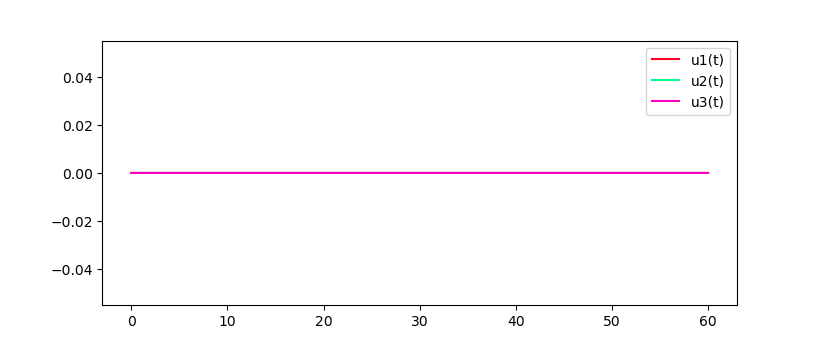
\includegraphics[width=\textwidth]{sol_p_0}
    \caption{Gráfica de \(\mathbf{u}(t)\) con \(\mathbf{P}(t) = \mathbf{0}\) para \(t \in [0, 60]\)}
    \label{fig:sol-p-0}
\end{figure}

En segundo lugar, consideramos una fuerza externa de la forma \(P_1(t) = m_1 a_g(t)\) ejercida sobre el primer piso. Esta tipo de función se utiliza para representar la fuerza ejercida sobre la base de una estructura durante un sismo \citep{kramer}, donde \(a_g(t)\) es la aceleración del suelo en función del tiempo. En particular, tomaremos \(a_g\) como una sinusoidal de la forma \(a_g(t) = A\sin(2\pi f t)\), donde \(A\) (en \(\si{m/s^2}\)) es la aceleración pico del suelo y \(f\) (en \(\si{Hz}\)) es su frecuencia de oscilación.

Tomando una aceleración pico de \(A = 0.3\) y frecuencia de oscilación de \(f = 4 \, \si{Hz}\), obtenemos la figura~\ref{fig:sol-sismo-corto}.

\begin{figure}[ht!]
    \centering
    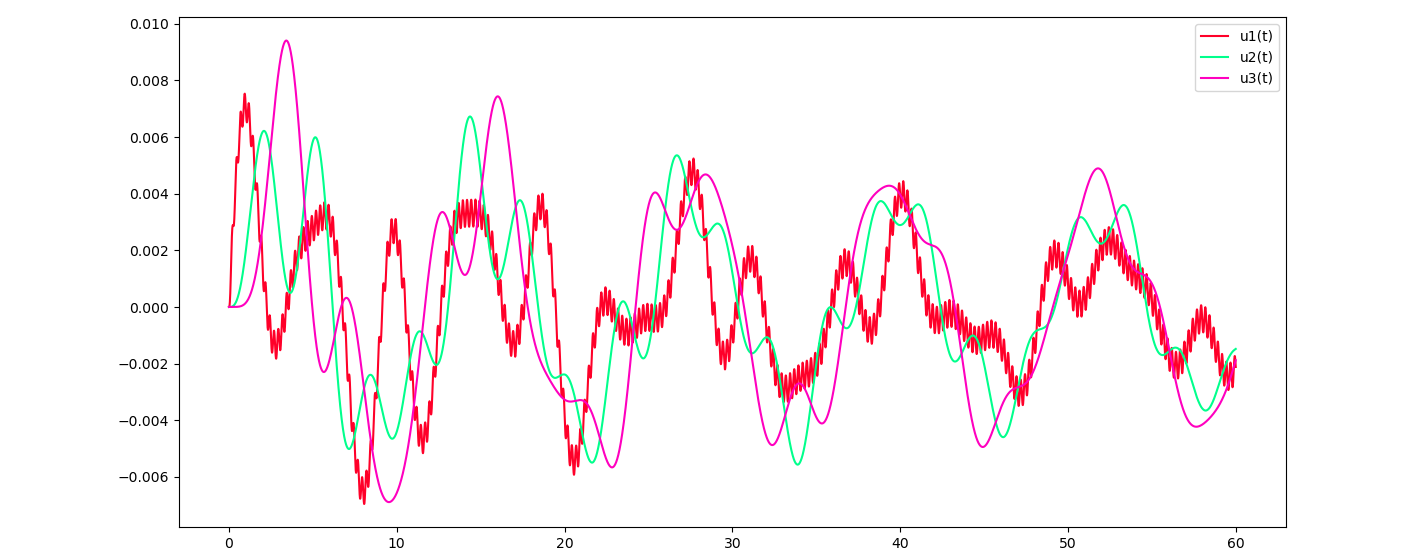
\includegraphics[width=\textwidth]{sol_sismo_corto}
    \caption{Gráfica de \(\mathbf{u}(t)\) con \(P_1(t) = m_1 A \sin(2\pi f t)\) para \(t \in [0, 60]\).}
    \label{fig:sol-sismo-corto}
\end{figure}

Sin embargo, se puede apreciar mejor el comportamiento a largo plazo de las vibraciones si extendemos la gráfica hasta un tiempo de 180 segundos (véase la figura~\ref{fig:sol-sismo-largo}).

\begin{figure}[ht!]
    \centering
    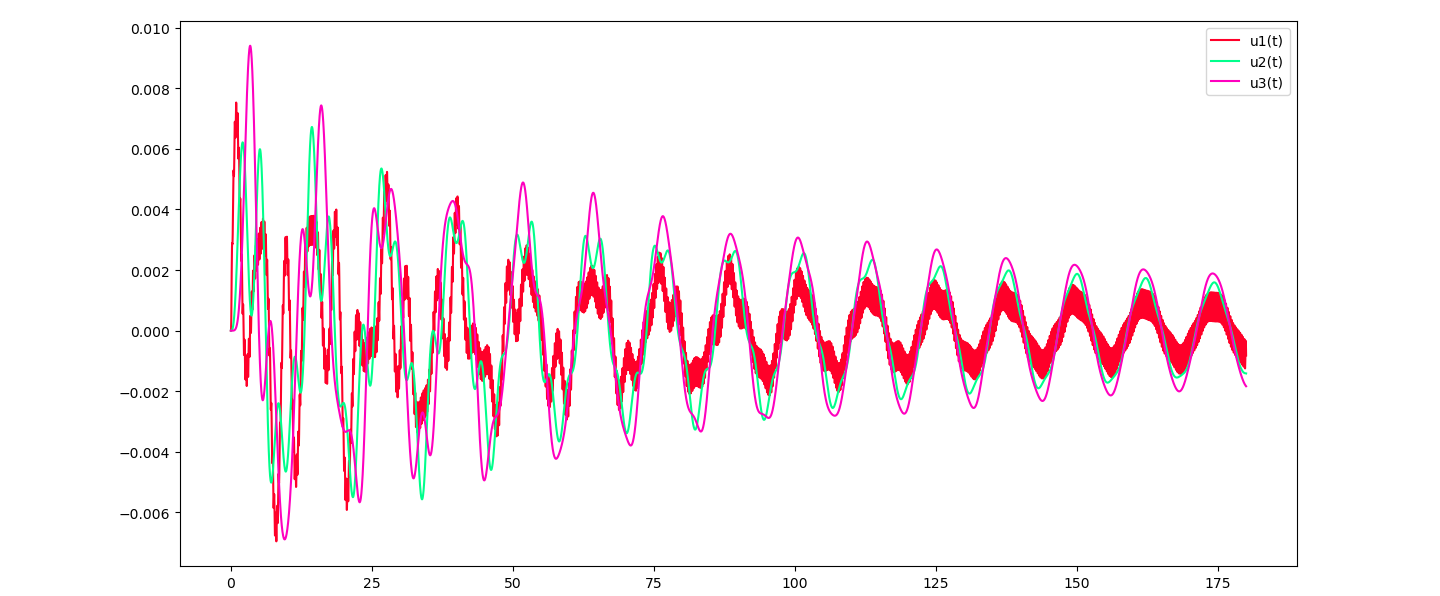
\includegraphics[width=\textwidth]{sol_sismo_largo}
    \caption{Gráfica de \(\mathbf{u}(t)\) con \(P_1(t) = m_1 A \sin(2\pi f t)\) para \(t \in [0, 180]\).}
    \label{fig:sol-sismo-largo}
\end{figure}

Si aumentamos las razones de amortiguamiento a
\[
    \zeta_1 = 10\%, \quad \zeta_2 = 5\%, \quad \zeta_3 = 2.5\%
,\]
se produce la figura~\ref{fig:sol-sismo-damped}. En esta gráfica, se puede notar que la amplitud de las vibraciones de la estructura se reduce más rápidamente que en la figura~\ref{fig:sol-sismo-largo}.

\begin{figure}[ht!]
    \centering
    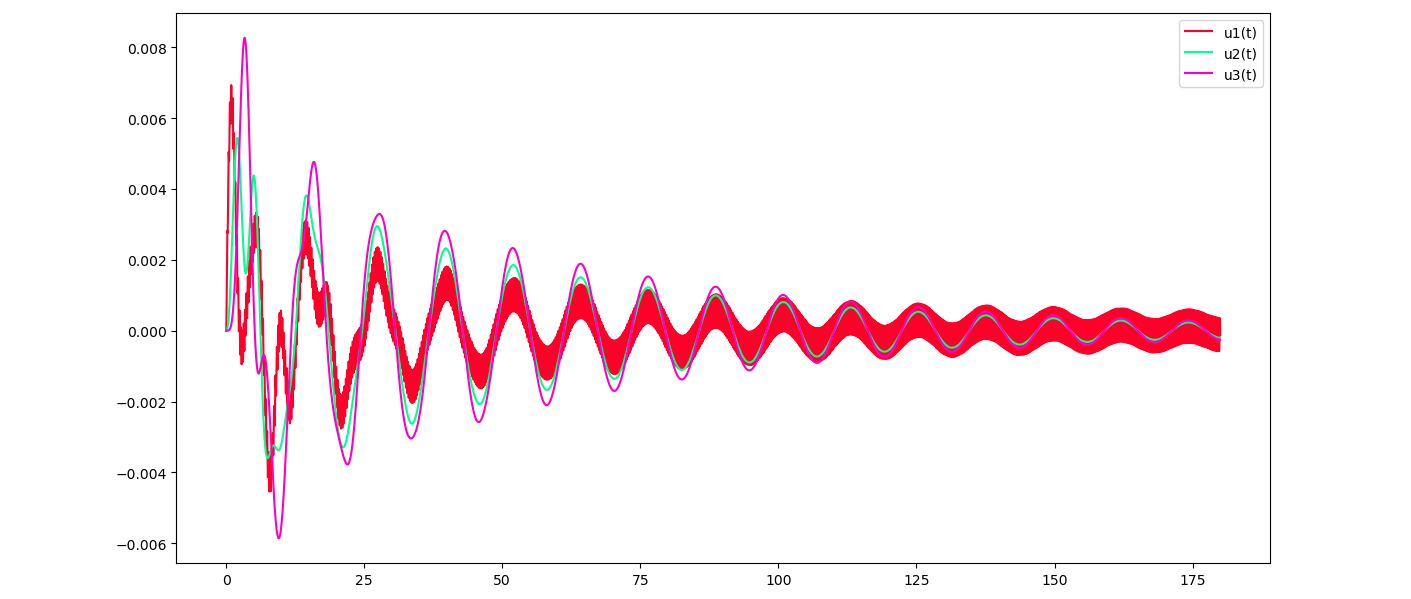
\includegraphics[width=\textwidth]{sol_sismo_damped}
    \caption{Gráfica de \(\mathbf{u}(t)\) con \(P_1(t) = m_1 A \sin(2\pi f t)\) para \(t \in [0, 180]\) (amortiguamiento aumentado).}
    \label{fig:sol-sismo-damped}
\end{figure}

Si, en lugar de aumentar el amortiguamiento, aumentamos los coeficientes elásticos a
\[
    k_1 = 200,000 \, \si{N/m}, \quad k_2 = 500,000 \, \si{N/m}, \quad k_3 = 800,000 \, \si{N/m}
,\]
se obtiene la figura~\ref{fig:sol-sismo-elastic}.

\begin{figure}[ht!]
    \centering
    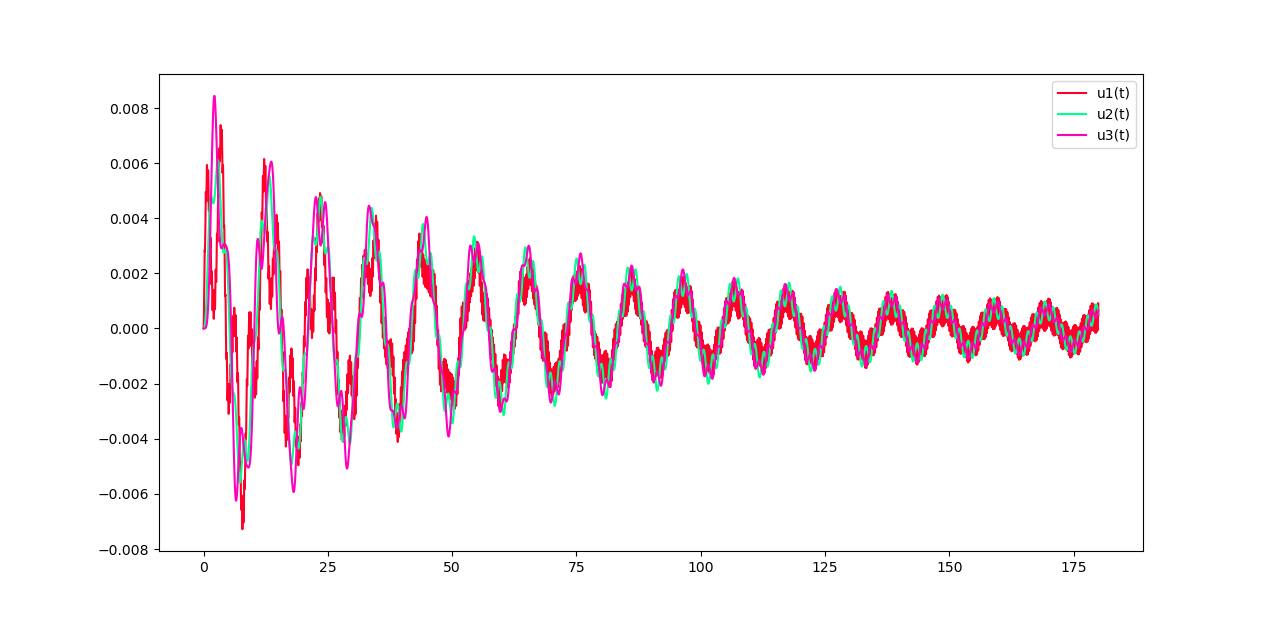
\includegraphics[width=\textwidth]{sol_sismo_elastic}
    \caption{Gráfica de \(\mathbf{u}(t)\) con \(P_1(t) = m_1 A \sin(2\pi f t)\) para \(t \in [0, 180]\) (elasticidad aumentada).}
    \label{fig:sol-sismo-elastic}
\end{figure}

\section{Análisis y discusión de la solución}
\section{Conclusiones}

El presente trabajo ha mostrado el modelado de un sistema de ecuaciones diferenciales para las vibraciones estructurales de una estructura de \(n\) pisos, y ha resuelto dicho sistema considerando diferentes conjuntos de parámetros. De esta manera, se han obtenido varias gráficas que muestran el comportamiento de los pisos de la estructura mientras que son sometidos a fuerzas externas a través del tiempo.

Por lo tanto, este informe presenta las siguientes conclusiones:

\begin{enumerate}
    \item Es posible modelar las ecuaciones diferenciales para el desplazamiento horizontal de los pisos de una estructura mediante el uso de la ley de Hooke, la ley de Newton y realizando ciertas suposiciones sobre el amortiguamiento que recibe cada piso. El proceso para modelar una estructura de \(n\) pisos se puede obtener directamente de tomar un modelo para 3 pisos y tomar a su segundo piso como un piso intermedio cualquiera del modelo de \(n\) pisos.

    \item Aunque es posible, en teoría, emplear métodos analíticos como la transformada de Laplace para resolver sistemas de ecuaciones de segundo orden como aquel planteado en este informe, en la práctica resulta extremadamente largo, tedioso y propenso a errores obtener respuestas analíticas con estos métodos.

    \item Los métodos numéricos, aunque no proveen soluciones analíticas a las ecuaciones diferenciales, constituyen una forma efectiva de obtener resultados de gran utilidad. En particular, son de gran apoyo cuando no es necesario explorar la naturaleza matemática de las soluciones, sino que, por ejemplo, baste con observar las gráficas que pueden producir.

    \item El modelado y resolución de ecuaciones diferenciales para estructuras de varios pisos (como puentes) es una forma práctica de simular y predecir el comportamiento de estas estructuras cuando se someten a fuerzas externas como sismos. Por ejemplo, se puede utilizar para determinar y analizar los efectos de la frecuencia natural de la estructura. Aunque el modelo presentado en este informe hace ciertas simplificaciones sobre el entorno físico de la estructura, igualmente puede ser efectivo para predecir comportamientos a corto plazo.
\end{enumerate}

Como se mencionó en la sección de propuestas prácticas de aplicación, este trabajo muestra un procedimiento que permite predecir el comportamiento de estructuras de \(n\) grados de libertad, al menos bajo ciertas suposiciones ideales sobre el entorno. Las gráficas que este método puede producir pueden ser de utilidad para observar los rangos de oscilación de los pisos de la estructura, experimentar con los efectos que genera variar los parámetros usados, y determinar un valor aproximado para la frecuencia natural de una estructura.

De la misma manera, se proponen las siguientes recomendaciones para trabajos de investigación a futuro en el tema:

\begin{enumerate}
    \item Para el modelado de sismos, considerar información empírica sobre vibraciones sísmicas para la construcción de funciones de fuerza externa \(\mathbf{P}(t)\). Aunque las funciones sinusoidales son una aproximación factible para la fuerza ejercida por el suelo sobre una estructura, lo óptimo sería poder utilizar una grabación de vibraciones sísmicas de la vida real. Dado que en este informe se utiliza un método numérico iterativo, la implementación de un modelo como este sería sencillo.

    \item En general, trabajar con modelos menos simplificados para la estructura de \(n\) pisos. Una de las razones por las que el método de RK4 fue efectivo para este trabajo particular fueron las simplificaciones que se realizaron en la construcción del modelo (por ejemplo, ignorar las interacciones suelo-estructura y la posibilidad del uso de materiales no-lineales). Sin embargo, este modelo podría no ser lo suficientemente confiable para realizar predicciones más críticas o para mayores rangos de timepo.
\end{enumerate}


\printbibliography[title=Bibliografía, heading=bibnumbered]

\begin{appendices}

\section{Sobre RK4 para sistemas de EDOs}\label{appendix:rk4-systems}

El método de Runge-Kutta de orden 4 se puede aplicar de forma análoga a su formulación original para resolver sistemas de ecuaciones diferenciales de primer orden. Es fácil observar que las ecuaciones presentadas en el marco teórico sobre Runge-Kutta pueden tomar a \(y\), \(f(x, y)\) y a los coeficientes \(k_i\) como vectores en el sistema de EDOs
\[
    \mathbf{y}'(x) = \mathbf{f}(x, \mathbf{y})
\]
de la siguiente manera:

\[
    \mathbf{y}_{n+1} = \mathbf{y}_n + \frac{1}{6}h(\mathbf{k}_1 + 2\mathbf{k}_2 + 2\mathbf{k}_3 + \mathbf{k}_4), x_{n+1} = x_n + h
,\]
y
\begin{align*}
    \mathbf{k}_1 &= \mathbf{f}(x_n, \mathbf{y}_n) \\
    \mathbf{k}_2 &= \mathbf{f}(x_n + \frac{1}{2}h, \mathbf{y}_n + \frac{1}{2}h\mathbf{k}_1) \\
    \mathbf{k}_3 &= \mathbf{f}(x_n + \frac{1}{2}h, \mathbf{y}_n + \frac{1}{2}h\mathbf{k}_2) \\
    \mathbf{k}_4 &= \mathbf{f}(x_n + h, \mathbf{y}_n + h\mathbf{k}_3)
.\end{align*}


\section{Código de Python utilizado}\label{appendix:rk4-code}

El código de Python utilizado en este informe para resolver \eqref{eqn:rk4-ready} con Runge-Kutta de orden 4 es el siguiente:

\inputminted{python}{./rk4.py}

Las líneas 43-54 contienen los parámetros del sistema de ecuaciones (masas, constantes de amortiguamiento y elasticidad, etc).

\section{Sobre la frecuencia natural de una estructura}\label{appendix:natural-frequency}

Cualquier estructura que corresponda al modelo que se presenta en este informe tiene una \textbf{frecuencia natural}. Se trata de una frecuencia particular a la que la estructura tiende a oscilar cuando no se le aplican fuerzas externas (es decir, cuando \(\mathbf{P}(t) = \mathbf{0}\)). Lo especial de esta frecuencia es que, de ser aplicada a la estructura una fuerza oscilatoria de frecuencia muy cercana o igual a su frecuencia natural , las oscilaciones de la estructura rápidamente ganarán mayor amplitud. Este fenómeno, conocido como \text{resonancia}, puede llevar a daños catastróficos, razón que motiva enormemente el estudio de esta propiedad en estructuras \citep{hernandez}.

Para encontrar la frecuencia natural de la estructura con los parámetros \eqref{eqn:sol-sismo-params}, generamos una gráfica con \(\mathbf{P}(t) = \mathbf{0}\) y condiciones iniciales \(\mathbf{u}(0) = \mathbf{1}\) (donde \textbf{1} denota un vector de 1s) y \(\mathbf{u}'(0) = \mathbf{v}(0) = \mathbf{0}\) (véase figura~\ref{fig:sol-natural-frequency}). En otras palabras, simulamos las oscilaciones que ocurrirían suponiendo que los pisos partiesen de un desplazamiento inicial de 1 metro a la derecha sin ser sometidos a fuerzas externas.

\begin{figure}[ht!]
    \centering
    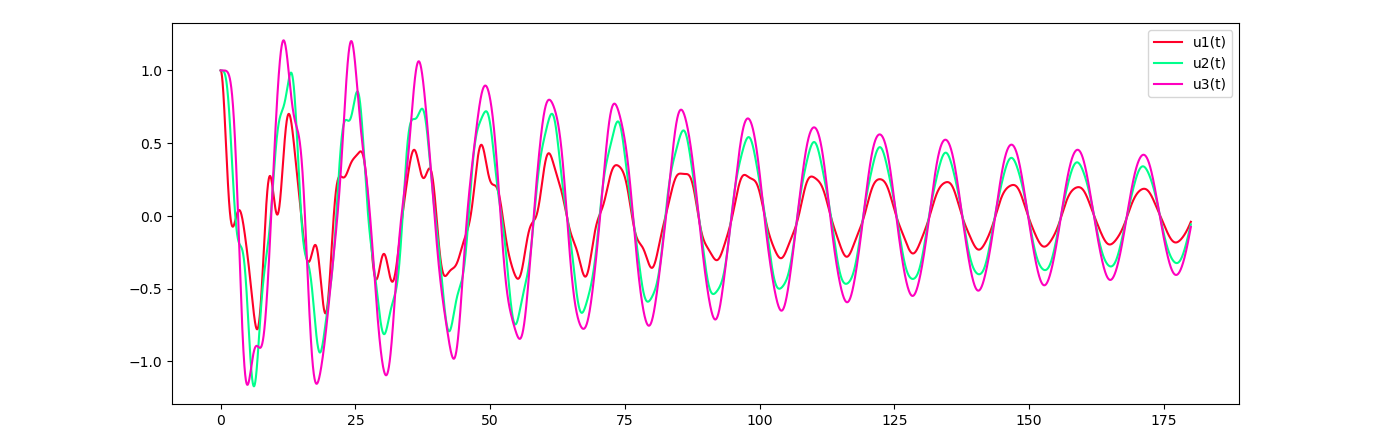
\includegraphics[width=\textwidth]{sol_sismo_natural_frequency}
    \caption{Gráfica de \(\mathbf{u}(t)\) con \(\mathbf{P}(t) = \mathbf{0}\) y condiciones iniciales \(\mathbf{u}(0) = \mathbf{1}\) para \(t \in [0, 180]\)}
    \label{fig:sol-natural-frequency}
\end{figure}

De la gráfica, contamos la cantidad de oscilaciones completas realizadas (llámese \(N\)) y el tiempo transcurrido durante estas oscilaciones (llámese \(\Delta t\)), de tal forma que se pudiese calcular la frecuencia natural \(f_n\) de la estructura con una precisión aceptable mediante
\[
    f_n = \frac{N}{\Delta t}
.\]

De la figura~\ref{fig:sol-natural-frequency}, en particular, se pueden observar \(14\) oscilaciones completas en un lapso de \(\Delta t = 171\) segundos, por lo que la frecuencia natural de la estructura mostrada, en particular, resulta
\[
    f_n = \frac{14}{171} \, \si{Hz} \approx 0.0819 \, \si{Hz}
.\]

\end{appendices}


\end{document}
